\documentclass[a4paper,12pt]{report}
\usepackage{preamble}

\author{Oscar Van Slijpe}
\title{Physical layer security:\\authentication and ciphering using physical unclonable functions on FPGA}

% Promotor, co-promotor, advisors, 
\promotor{Dr. Pr. Jean-Michel Dricot}
\advisors{Dr. Pr. Dragomir Milojevic}
\reason{Electronics and Information Technology \\ Engineering}
\AcademicYear{2022-2023}


\begin{document}
\frontmatter
% Title page
\maketitlepage

\begin{figure}
    \centering
    
\includegraphics[width=\linewidth]{images/ulb.png}
\end{figure}

\subsection*{Reserve au secretariat}

Memoire reussi\footnote{Biffer la mention inutile} \textbf{OUI NON}\\

\vspace{0.5cm}

\hline

\vspace{0.5cm}

\subsection*{Consultation du memoire/travail de fin d'etudes}


\noindent Je soussigne\\

\begin{minipage}[b]{0.05\linewidth} 
\end{minipage}\hfill
\begin{minipage}[b]{0.95\linewidth}   
\textbf{NOM :} \textit{VAN SLIJPE}\\
\textbf{PRENOM :} \textit{OSCAR}\\
\textbf{TITRE DU TRAVAIL} : \textit{Physical layer security: authentication and ciphering using physical unclonable functions on FPGA}\\
\end{minipage}



\noindent\textbf{AUTORISE \sout{REFUSE}} la consultation du present memoire/travail de fin d'etudes par les utilisateurs des bibliotheques de l'Universite libre de Bruxelles.\\

Si la consultation est autorisee, le soussigne concede par la presente a l'Universite libre de Bruxelles, pour toute la duree legale de protection de l'oeuvre, une licence gratuite et non exclusive de reproduction et de communication au public de son oeuvre precisee ci-dessus, sur supports graphiques ou electroniques, afin d'en permettre la consultation par les utilisateurs des bibliotheques de l'ULB et d'autres institutions dans les limites du pret inter-bibliotheques.\\

Fait en deux exemplaire, \textbf{Bruxelles}, le \textit{21/08/2023}\\
\textbf{Signature}

\chapter*{Abstract}
\addcontentsline{toc}{chapter}{Abstract}

\acrfull{puf} is a promising way to redefine how we implement security in modern systems. \acrfull{teropuf} is a recent method that shows good performance with compact design. In this work, we propose two \acrshort{teropuf} implementations on Artix-7 \acrfull{fpga}, the first using one slice per cell and the second using one \acrfull{clb} per cell. The more compact one doesn't reach state of the art performance, while the second gives performance similar to the existing \acrshort{teropuf} implementation on other devices. This shows the limitations of the size of this \acrshort{puf}. We make use of \acrfull{ecc} to further improve the reliability of the response, and we have added a \acrfull{sha} to generate a key that can be used for encryption demonstration.\\

\textbf{Keywords:} \acrlong{puf}; \acrlong{teropuf}; \acrlong{fpga}; Artix-7; Secure hardware design; Cryptographic primitive

\vspace*{\fill}\\
\noindent Oscar Van Slijpe\\
Electronics and Information Technology Engineering\\
Physical layer security: authentication and ciphering using physical unclonable functions on FPGA\\
2022-2023

%Demonstrator motivation

%Generic electronic
\newacronym{ic}{IC}{Integrated Circuit}
\newacronym{mux}{MUX}{Multiplexer}
\newacronym{sram}{SRAM}{Static Random-Access memory}
\newacronym{fpga}{FPGA}{Field-Programmable Gate Array}
\newacronym{lut}{LUT}{Look-Up Table}
\newacronym{clb}{CLB}{Configurable Logic Block}
\newacronym{sr-latch}{SR-Latch}{Set-Reset Latch}
\newacronym{prng}{PRNG}{Pseudo-Random Number Generator}
\newacronym{trng}{TRNG}{Truly-Random Number Generator}
\newacronym{ml}{ML}{Machine Learning}
\newacronym{vhdl}{VHDL}{VHSIC Hardware Description Language}
\newacronym{lsfr}{LSFR}{Linear Shift Feedback Register}
\newacronym{xdc}{XDC}{Xilinx Design Constraints}
\newacronym{sha}{SHA}{Secure Hash Algorithm}
\newacronym{bch}{BCH}{Bose Chaudhuri and Hocquenghem code}
\newacronym{uart}{UART}{Universal Asynchronous Receiver Transmitter}
\newacronym{pll}{PLL}{Phase-locked loop}
\newacronym{ecc}{ECC}{Error Correction Code}
\newacronym{ber}{BER}{Bit Error Rate}
\newacronym{bst}{BST}{Bit-Self Test}
\newacronym{nist}{NIST}{National Institute of Standards and Technology}
\newacronym{aes}{AES}{Advanced Encryption Standard}
\newacronym{ip}{IP}{Intellectual property}
\newacronym{iot}{IoT}{Internet of Things}

%Generic PUF
\newacronym{puf}{PUF}{Physical Unclonable Function}
\newacronym{powf}{POWF}{Physical One-Way Function}
\newacronym{sprf}{SPRF}{Silicon Physical Random Function}
\newacronym{spuf}{SPUF}{Silicon PUF}
\newacronym{crp}{CRP}{Challenge-Response Pair}

%PUF types
\newacronym{apuf}{APUF}{Arbiter PUF}
\newacronym{ffapuf}{FF-APUF}{Feed-Forward Arbiter PUF}
\newacronym{xorapuf}{XOR-APUF}{XOR Arbiter PUF}
\newacronym{bstapuf}{BST-APUF}{Bit-Self Test Arbiter PUF}
\newacronym{ropuf}{RO-PUF}{Ring Oscillator PUF}
\newacronym{mropuf}{M-ROPUF}{Mux-based Ring Oscillator PUF}
\newacronym{teropuf}{TERO-PUF}{Transient Effect Ring Oscillator PUF}
\newacronym{tero}{TERO}{Transient Effect Ring Oscillator}
\newacronym{ocpuf}{OC-PUF}{Oscillator Collapse PUF}
\newacronym{ddpuf}{DD-PUF}{Delay Differential PUF}
\newacronym{srampuf}{SRAM-PUF}{SRAM PUF}
\newacronym{rwcsrampuf}{RWC-SRAMPUF}{Read-Write Collision SRAM-PUF}
\newacronym{bpuf}{BPUF}{Butterfly PUF}
\newacronym{ffpuf}{FFPUF}{Flip-Flop PUF}

%Metrics
\newacronym{relia}{RE}{Reliability}
\newacronym{unif}{UF}{Uniformity}
\newacronym{uniq}{UQ}{Uniqueness}
\newacronym{bit-alia}{BA}{Bit-Aliasing}




\printglossary[type=\acronymtype, title={List of Acronyms}, toctitle={List of Acronyms}]


\setcounter{tocdepth}{2}
\tableofcontents

\newpage
\mainmatter

%Lecteur can read chap 1 -> result and be ok !



\chapter{Introduction}

%ARCHITECTURE
%General context and knowledge
With the advent of new technologies such as \acrfull{iot} or Smart Grid, there is an increasing amount of data being collected and transmitted between devices that could be physically available to anyone, and which sometimes cannot be secured using classical security techniques due to the small computing resources available. Therefore, alternative security methods where a device is able to generate its own security, with a system that has a small footprint compared to its main system, are highly desirable.\\

%Introduce the problem to be solved
One promising candidate, \acrshort{puf}, are physical systems that cannot be replicated identically even if you know exactly how they were created. This means that the output of the function is determined by some intrinsic properties of the system itself, which either cannot be known or cannot be manufactured with sufficient accuracy to give the same responses. Furthermore, if these unknown properties are random, then the response to a given input will also appear to be completely random. The responses are extracted from the system itself and not stored in some kind of internal memory, making them less accessible.\\

\acrshort{puf}s have been studied in various forms since 2001 \cite{pappu_physical_2001} and there are some applications using them such as \acrfull{ip} protection for \acrshort{fpga} \cite{paillier_fpga_2007}, authentication protocols for \acrshort{iot} \cite{al-meer_physical_2022, ebrahimabadi_attack_2022, bendavid_iot_2018} or security for chiplet devices \cite{deric_know_2022}.\\

%Already mention the contribution of this study (scientific + demonstration)
In this work, we present an implementation of a \acrfull{teropuf} for the first time on Artix-7, with state-of-the-art performance and the possibility to generate a usable key using \acrshort{sha}. The different design possibilities are discussed and two implementations are tested to compare the effect of the size of the \acrshort{tero} cells.







\chapter{Physical Unclonable Function: classification and characterisation}
\label{ch:1-puf}


In this section, we will discuss in more detail about the typical design of \acrshort{puf}, how they work, and how we can evaluate their performance.

\begin{figure}[H]
    \centering
    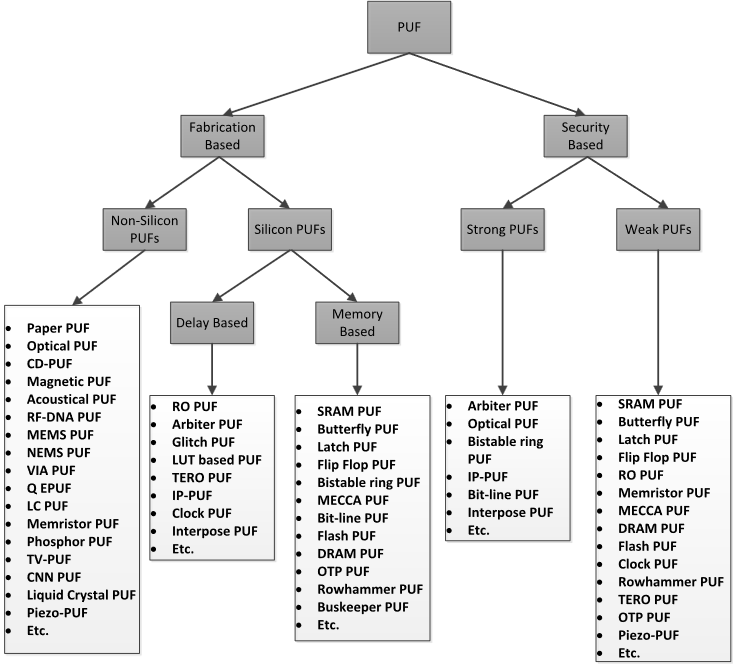
\includegraphics[width=0.84\linewidth]{images/full_puf_overview.png}
    \caption{\acrshort{puf} classification (from~\cite{anandakumar_fpga-based_2021})}
    \label{fig:PUF_ALL}
\end{figure}

The \acrshort{puf} concept was introduced in 2001 by \cite{pappu_physical_2001, pappu_physical_2002}, first addressed as \acrfull{powf}, as a comparison to the one-way functions based on number theory used in cryptography. The aim is to exploit randomness in the physical properties of a system to generate a binary sequence. As a first proof of concept, they used a transparent epoxy containing bubbles as the physical medium, which was 'read' by a laser at a specific angle to generate a pattern from the interference between the beam and the epoxy/bubble.\\

This has led to a variety of different designs which can be classified in two ways, as shown in figure~\ref{fig:PUF_ALL}: how they work physically (manufacturing based) and how they should be used (safety based).

\section{Fabrication based classification}

%FPAG-based \acrshort{puf} -> Also good for security

The non-silicon \acrshort{puf}s are \acrshort{puf}s implemented on systems such as optical, mechanical or magnetic systems. These will not be covered in this study and we will concentrate only on \acrfull{spuf}. The first introduction of \acrshort{spuf} was made by \cite{gassend_silicon_2002} in 2002, originally called \acrfull{sprf}. The advantage of such \acrshort{puf}s is the ease with which they can be integrated into other electronic circuits.\\

In general, electronic circuit models are expected to have some small number of defects in the silicon due to the limited precision of the manufacturing process. The defects are required to have a negligible effect on the device's operation, and this is a constraint that designers consider while designing such circuits. However, these effects can still be exhibited using appropriately designed circuits. These defects cannot be replicated with a similar precision manufacturing process and are often considered to be unknowable (in the sense that to be able to observe them directly one would generally need to destroy the \acrfull{ic}) and appear to be random. This means that they are properties that can be used to implement a \acrshort{puf} on an electronic circuit.\\

A wide range of methods can be utilised to expose these tiny manufacturing errors and to turn them into usable responses, i.e. binary values. There are two classes of methods based on how they exploit randomness: delay-based \acrshort{puf} and memory-based \acrshort{puf}. Designs using more than one \acrshort{puf} technique are called hybrid \acrshort{puf}.\\

Delay-based \acrshort{puf}s exploit small variation in the delay of electronic signals between two similar paths. In an ideal scenario, the two paths should produce identical delays, but in reality, there will always be slight differences in delay. These differences are typically small, and their influence on a typical electronic circuit is minimal. Delay-based \acrshort{puf} are electronic circuits designed to amplify these differences to the point where they dominate and determine the output response, ideally without any other external factor influencing the result.\\

Memory-based \acrshort{puf}s exploit transient state of memory elements during power-up and then observe which stable states they eventually transition to, resulting in the generation of the response.\\


\section{Security based classification}

A second way of classifying \acrshort{puf} is to separate them on the basis of the size of their \acrfull{crp} space. Some \acrshort{puf}s provide only one possible response. In this case, it can be considered that there is no input since the challenge corresponding to the only response is intrinsic to the \acrshort{puf} itself. Whereas, other \acrshort{puf}s have a large set of \acrfull{crp} spaces. This classification is helpful in determining how a \acrshort{puf} can be utilized for security applications.\\

Weak \acrshort{puf} are the \acrshort{puf}s with a small \acrshort{crp} space, with the extreme case being a \acrshort{puf} with only one response (the challenge is therefore not required as an input, as it is implicit in the \acrshort{puf} itself). These \acrshort{puf}s must be used in a secure environment and the \acrshort{crp} should not be revealed; otherwise, an attacker could record the entire CRP, compromising the security of the system. Thefore, these \acrshort{puf}s can only be used for applications such as key extraction, truly random number generation, or identification.\\

Strong \acrshort{puf} refers to \acrshort{puf}s with a large \acrshort{crp} space. In this case, revealing a few \acrshort{crp} does not compromise the \acrshort{puf} because there are still many of them that are unknown (in the ideal case where \acrshort{crp}s are not correlated in any way so that the remaining \acrshort{crp} cannot be predicted). Strong PUFs are ideal for use in authentication processes.


\section{Example of FPGA-based PUFs}


\subsection{Arbiter PUF}

\acrfull{apuf} are the most common and most studied of the \acrshort{puf}s.\\
The concept was introduced in 2002 \cite{gassend_silicon_2002} and many different versions have been created since then. It consists of two paths that travel through successive stages, where the 2 paths have 2 possible configurations depending on the input. The output is generated based on which path is globally the fastest due to the imperfections in the IC. This can be achieved by using successive stages of \acrfull{mux} that select which path the signal will take, as shown in figure~\ref{fig:APUF}.\\
Thus, this is a delay-based \acrshort{puf}, and since the number of \acrshort{crp} doubles for each additional stage, it is a strong \acrshort{puf}.

\begin{figure}[H]
    \centering
    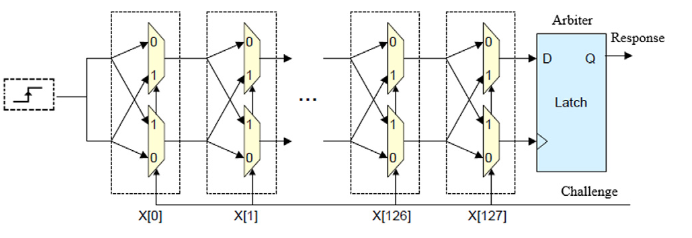
\includegraphics[width=0.75\linewidth]{images/APUF_diagram.png}
    \caption{Arbiter \acrshort{puf} diagram \cite{anandakumar_fpga-based_2021}}
    \label{fig:APUF}
\end{figure}

One concern with this design is the possibility to model the internal delay of each stage configuration to be able to predict the entire \acrshort{crp} space. A proposed countermeasure for this issue was presented in 2004 \cite{lee_technique_2004}, where feed-forward signals from the intermediate stage are used as input for some of the following stages. This approach is commonly known as a \acrfull{ffapuf}.\\

\begin{figure}[H]
   \begin{minipage}[b]{0.6\linewidth} 
        \centering
        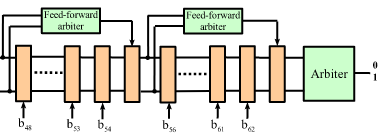
\includegraphics[width=\linewidth]{images/FF-APUF_Lee and al 2004.png}
        \caption{\acrshort{ffapuf} \cite{lee_technique_2004}}
        \label{FFAPUF}
   \end{minipage}\hfill
   \begin{minipage}[b]{0.35\linewidth}   
        \centering
        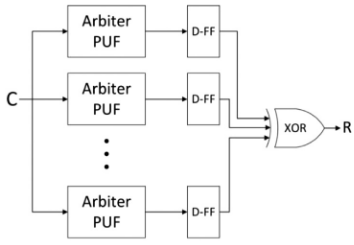
\includegraphics[width=\linewidth]{images/XOR-APUF Al-Hajj and al. 2021.png}
        \caption{\acrshort{xorapuf} \cite{el-hajj_taxonomy_2021}}
         \label{XORAPUF}
   \end{minipage}
\end{figure}

An alternative approach is to introduce an XOR layer at the output to enhance the confidentiality of the internal properties. This was studied by \cite{suh_physical_2007} in 2007, called a \acrfull{xorapuf}.\\

Since then, several other features have been developed and tested. To enhance the reliability, \cite{he_highly_2020} has proposed a \acrfull{bstapuf}. A more recent example is the work of \cite{anandakumar_implementation_2022} in 2022, which obfuscates the challenges and adds a majority voting system before the XOR. A comprehensive compilation of Arbiter \acrshort{apuf} was done by \cite{el-hajj_taxonomy_2021} in 2021.



\subsection{Ring oscillator PUF}

The design proposed by \cite{gassend_silicon_2002} does not directly evaluate the delay difference between two configurable paths. Rather, the signals were looping back into the same configurable path, thus forming an oscillating circuit. The frequency difference served as the measured parameter for determining the output. This was done in order to reduce the influence of the process variation on the output parameter.\\

\begin{figure}[H]
    \centering
    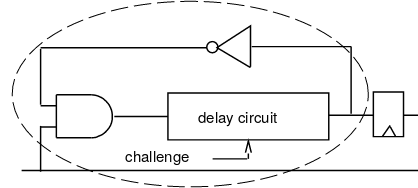
\includegraphics[width=0.6\linewidth]{images/RO_origine_Gassend_al_2002.png}
    \caption{Oscillating circuit using APUF for delay \cite{gassend_silicon_2002}}
    \label{fig:RO_ORIGINAL}
\end{figure}

This concept led to the development of another \acrshort{puf} design: the \acrfull{ropuf}. An oscillating circuit is designed using a basic delay element and replicated to form a collection of oscillators. All oscillators are compared to each other, and a '0' or a '1' is generated based on the oscillator with the fastest frequency.

\begin{figure}[H]
    \centering
    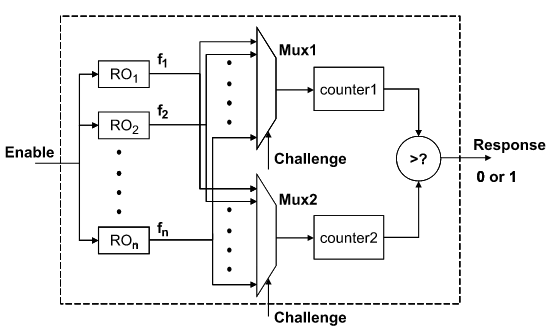
\includegraphics[width=0.7\linewidth]{images/RO_GENE_ORIGI_maiti_2009.png}
    \caption{\acrshort{ropuf} diagram \cite{maiti_improved_2009}}
    \label{fig:ROPUF}
\end{figure}

This concept was first studied in 2009 by \cite{maiti_improved_2009} using a \acrshort{sram} based \acrshort{fpga} (Spartan 3), then in 2017 by \cite{mureddu_efficient_2017} with a flash based \acrshort{fpga} (Microsemi SmartFusion2). In both cases, the oscillator circuit is made up of an AND gate (for control) and an odd number of NOT gates (for delay).\\

In 2022, \cite{yao_m-ro_2022} demonstrated the possibility of replacing the inverter-based oscillator with a \acrshort{mux}-based one, resulting in the creation of the \acrfull{mropuf}.

\begin{figure}[H]
    \centering
    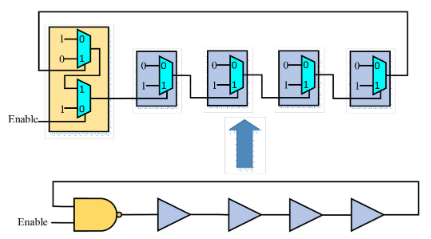
\includegraphics[width=0.7\linewidth]{images/MUX_ROPUF_YAO.png}
    \caption{\acrshort{mropuf} \cite{yao_m-ro_2022}}
    \label{fig:MUXROPUF}
\end{figure}

Similarly to the \acrshort{apuf}, \acrshort{ropuf} are delay-based \acrshort{puf}s. They can be considered weak or strong \acrshort{puf} depending on the oscillator circuit designs as well as the structure used to generate the output from the collection of oscillators.


%ResumeHere

\subsection{Transient effect ring oscillator PUF}
\label{subsubsec:intr_tero_puf}

The \acrshort{ropuf} concept has been proven to be often very vulnerable to physical attack and frequency analysis by \cite{clavier_frequency_2009} in 2009, \cite{bochard_true-randomness_2010} in 2010, \cite{hutchison_contactless_2012} in 2012 and \cite{bossuet_ultra-lightweight_2015} in 2015. Moreover, \cite{bochard_true-randomness_2010} also proved that the different oscillator cells of \acrshort{ropuf} are sensitive to locking phenomena (cells are not independent).\\

To avoid the locking phenomena and make the frequencies less accessible, a new design using transient effect has been proposed by \cite{bossuet_puf_2014} in 2014.\\
In \acrfull{teropuf}, the cells oscillation occurs in an unstable state and both the stabilisation time and the final number of oscillations are unpredictable. This can be achieved with the circuit represented in figure~\ref{fig:TEROPUF}, which is an \acrfull{sr-latch} with the set and reset signal combined. This design is also sometimes called \acrfull{ocpuf}

\begin{figure}[H]
    \centering
    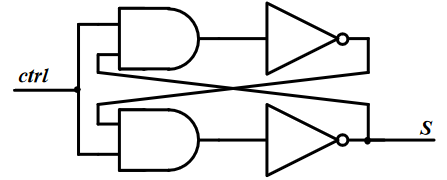
\includegraphics[width=0.5\linewidth]{images/TEROPUF.png}
    \caption{\acrshort{teropuf} diagram \cite{bossuet_puf_2014}}
    \label{fig:TEROPUF}
\end{figure}

The first design by \cite{bossuet_puf_2014} was tested on an Altera Cyclone II then by \cite{marchand_design_2016} on Altera Cyclone V and Xilinx Spartan 6 FPGAs.\\

The oscillator circuit has also been build using \acrshort{sr-latch} in \cite{habib_implementation_2017} and D-Latches in \cite{della_sala_novel_2021}, called \acrfull{ddpuf}.\\

\begin{figure}[H]
    \centering
    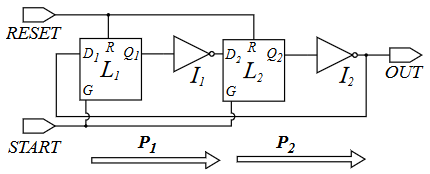
\includegraphics[width=0.5\linewidth]{images/DDPUF.png}
    \caption{\acrshort{ddpuf} diagram \cite{della_sala_novel_2021}}
    \label{fig:DDPUF}
\end{figure}

The idea of a programmable delay line using LUT input-output latency was re-introduced in 2018 by \cite{ardakani_improving_2018} on Spartan 3E and a high \acrshort{crp}s implementation ($2^{3N}$) has been proposed by \cite{zhang_highly_2020} in 2020 on an Altera DE2-115.\\

In 2019, \cite{tebelmann_side-channel_2019} studied the robustness of \acrshort{teropuf} design against side channels analysis. While it shows that \acrshort{teropuf} can still be vulnerable to some extent, it has also proposed a few countermeasures to minimise it. \acrshort{teropuf} still appear as one of the most promising delay based \acrshort{puf}.



\subsection{SRAM PUF}

In parallel to the evolution of delay based \acrshort{spuf}, the memory based \acrshort{spuf} development started with the \acrfull{srampuf} from \cite{paillier_fpga_2007} in 2007.\\
When an \acrshort{sram} element is powered up, its initial state is not one of the two stable ones ('1' and '0') but an unstable equilibrium in between. If none of the two stable states is forced, the state in which it will end up is unpredictable and is a function of the exact properties of the silicon.

\begin{figure}[H]
    \centering
    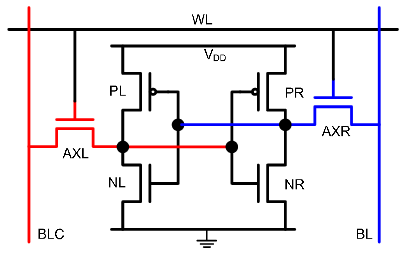
\includegraphics[width=0.45\linewidth]{images/SRAM.png}
    \caption{SRAM cell \cite{paillier_fpga_2007}}
    \label{fig:SRAM}
\end{figure}

This design has to advantage of using standard \acrshort{sram} chips, which are typically available in most of electronic board.\\
There have been multiple implementations since then, such as \cite{chen_fpga_2018} in 2008, who built a \acrfull{prng} from it, or \cite{usmani_applications_2018} in 2008 that used the variation of the \acrshort{puf} due to the temperature to create a temperature sensor with secured data values.\\


To eliminate the requirement of power up the \acrshort{sram} each time the \acrshort{puf} needs to be evaluated, \cite{cicek_new_2022} proposed in 2022 to introduce a \acrfull{rwcsrampuf}, violating in purpose the recommended operation of the \acrshort{sram}.


\subsection{Butterfly PUF}

For \acrshort{srampuf}, the \acrshort{fpga} needs to support uninitialised \acrshort{sram} memory, which is not always the case. To remove this requirement, \cite{kumar_extended_2008} introduced their \acrfull{bpuf} in 2008. The concept is the same that the \acrshort{srampuf} but the memory structure used is a cross-coupled latch that can be forced to an unstable state. 


\begin{figure}[H]
    \centering
    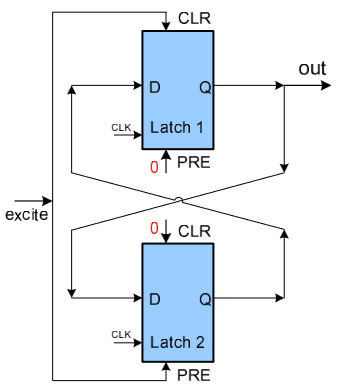
\includegraphics[width=0.45\linewidth]{images/BPUF.png}
    \caption{BPUF \cite{kumar_extended_2008}}
    \label{fig:BPUF}
\end{figure}


\subsection{Flip-Flop PUF}

Similarly to the \acrshort{bpuf}, the \acrfull{ffpuf} aims at removing the requirement on specific hardware from the \acrshort{srampuf}. Introduced in 2008 by \cite{maes_intrinsic_2008}, this \acrshort{puf} read the power-up value from D Flip-Flop.

\newpage
\subsection{Hybrid PUF}

It is also possible to combine two or more \acrshort{puf} techniques to have a more complex system that exploits the random defects in multiple ways. This can be useful to obtain a \acrshort{puf} that is more difficult to predict using \acrfull{ml} techniques. For example, \cite{devika_fpga_2022} has proposed in 2022 an implementation using both \acrshort{apuf} and \acrshort{bpuf} together.

\begin{figure}[H]
    \centering
    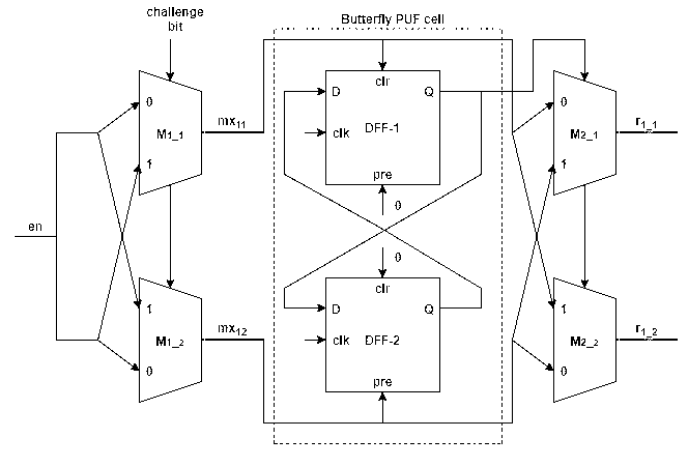
\includegraphics[width=\linewidth]{images/hybrid.png}
    \caption{Hybrid \acrshort{puf} diagram \cite{devika_fpga_2022}}
    \label{fig:HYBRID}
\end{figure}

\newpage
\section{Metrics}

To characterise and compare the performance of a \acrshort{puf}, multiple metrics have been used. In this section, we will see the main metrics used to evaluate the performance of \acrshort{puf} for security applications. The metrics that are computed on the set of responses of a single device are called intra-device metrics, and those that characterise the difference between the responses of different devices are called inter-device metrics.

\subsection{Uniformity}

The \acrfull{unif} is a measure of distribution between "0" and "1" bits in the response of a given device (intra-device). Ideally equal to 50\% to maximise the entropy.

\begin{equation}
    UF = \frac{1}{n} \sum_{i=1}^{n} r_i \times 100\%
\end{equation}

Where $n$ is the size of the response and $r_i$ is the $i$th bit of it.

\subsection{Reliability}


The \acrfull{relia} is a measure of the stability of the response of a given device (intra-device). Ideally equal to 100\% meaning that the response's bits are always the same.

\begin{equation}
     RE = 100\% - \frac{1}{s} \sum_{i=1}^s \frac{\mathrm{HD}\left(X_{ref}, X_i\right)}{n} \times 100 \% \\
\end{equation}

Where $s$ is the number of responses generated, $HD(X_{ref}, X_i)$ is Hamming distance between the $i$th response generated and the reference response.\\

The \acrfull{ber} can be obtained using only the right term of the sum.\\

This can be further improved using \acrfull{ecc} or \acrshort{bst} as done in \cite{he_highly_2020, he_highly_2021}.

\subsection{Bit-Aliasing}

The \acrfull{bit-alia} is a measure of how likely a bit value is to be '1' over all the devices (inter-device). This can reveal a bias in the implementation i.e. the response's bits are influenced by the implementation itself. Ideally, the distribution of bit-aliasing over different devices should follow a normal distribution centred around 50\%.

\begin{equation}
    BA_j = \frac{1}{k} \sum_{j=1}^{k} r_{i,j} \times 100\%
\end{equation}

Where $n$ is the number of bits of the response, $k$ is the number of devices and $r_{i,j}$ is the $i$th bit of the $j$th device response.

\subsection{Uniqueness}

The \acrfull{uniq} is a measure of how different the responses of different devices are (inter-device). Ideally equal to 50\%.

\begin{equation}
    UQ =\frac{2}{k(k-1)} \sum_{i=1}^{k-1} \sum_{j=i+1}^k \frac{\mathrm{HD}\left(X_i, X_j\right)}{n} \times 100\%
\end{equation}

Where $k$ is the number of devices, $\mathrm{HD}\left(X_i, X_j\right)$ the Hamming distance between the response word of device $i$ and $j$.


\newpage
\section{State of the art}
\label{sec:SOACompa}

The metrics just described are useful to compare the performance of different implementations. The table~\ref{tab:soa_impl} reports the performance of some of the \acrshort{fpga} implementation describes up to now. Not all studies have used the 4 metrics described here, and the implementations are done using different \acrshort{fpga}. The goal of this table is not to have a complete collection of \acrshort{puf}s implementation, only to have an overview of the typical performance that can be reached currently.\\

\begin{table}[H]
    \centering
    \begin{tabular}{|c|c|c|c|c|c|c|c|}
         \hline
         \textbf{method} & \textbf{\acrshort{relia}} & \textbf{\acrshort{unif}} & \textbf{\acrshort{uniq}} & \textbf{\acrshort{bit-alia}} & \textbf{device} & \textbf{Ref}\\
         \hline\hline
         \acrshort{apuf} & 99.55\% & 51.84\% & 46.21\% & -  & Artix-7 & \cite{anandakumar_implementation_2022}\\
         \hline
         \acrshort{ffapuf}& 90.2\% & - & 38\% & - & ASIC & \cite{lee_technique_2004}\\
         \hline
         \acrshort{xorapuf} & 99.41\% & 50.73\% & 48.69\% &  - & Artix-7 & \cite{anandakumar_implementation_2022}\\
         \hline
         \acrshort{bstapuf} & 99.99\% & - & 49.1\% & 50.3\% &  Artix-7 & \cite{he_highly_2020}\\
         \hline
         \acrshort{ropuf} & 100\% & - & 45.9\% & - &  Spartan-3 & \cite{maiti_improved_2009}\\
         \hline
         \acrshort{ropuf} & 99.19\% & 51.01 & 47.86\% & 51.01\% & Artix-7 & \cite{de_weerdt_implementation_2021}\\
         \hline
         BST-\acrshort{ropuf} & 99.99\% & 46.78\% & 48.64\% & - & Artix-7 & \cite{he_highly_2021}\\
         \hline
         \acrshort{mropuf} & - & 51.17\% & 49.52\% & 54.41\% & Kintex-7 & \cite{yao_m-ro_2022}\\
         \hline
         \acrshort{teropuf} & 97.4\% & - & 48.5\% & - & Spartan-6 & \cite{marchand_implementation_2017}\\
          & 98.2\% & - & 47.6\% & - & Cyclone-V & \cite{marchand_implementation_2017}\\
         \hline
         PDL-\acrshort{teropuf} & 98.8\% & - & 49.32\% & - & Spartan-3 & \cite{ardakani_improving_2018}\\
         \hline
         \acrshort{srampuf} & 98.2\% & - & - & - & Virtex-7 & \cite{usmani_applications_2018}\\
         \hline
         \acrshort{rwcsrampuf} & 98.92\% & 55.38\% & 37.36\% & 46.89\% & Artix-7 & \cite{cicek_new_2022}\\
         \hline
         \acrshort{ffpuf} & ~99\% & 49.2\% & - & 48.96\% & Artix-7 & \cite{khan_symmetric_2020}\\
         \hline
         
    \end{tabular}
    \caption{\acrshort{puf} implementations on \acrshort{fpga}}
    \label{tab:soa_impl}
\end{table}




%Separate state of the art and metric/classification

%title: Physical unclownable function, concept, state of the art...

%Focus to show what this study add !
%Motivate your contribution and explain more precisly the contribution

\chapter{Objectives}

Different \acrshort{puf}s methods were described in chapter~\ref{ch:1-puf}. In particular, we saw the evolution of delay-based \acrshort{spuf} from \acrshort{apuf} to \acrshort{teropuf}. While \acrshort{apuf} has been studied multiple times, on different devices with diverse variations, \acrshort{teropuf} is more recent and only some devices and variations have been studied until now.\\

Therefore, this thesis proposes a \acrshort{teropuf} implementation on Artix-7 and tested on 33 boards (Basys-3), which, as far as we know, is lacking to this day. Furthermore, we aimed at a design that can easily be used to demonstrate the \acrshort{puf} usage for ciphering.\\

This work follows the one from~\cite{de_weerdt_implementation_2021} in 2021 who studied an \acrshort{ropuf} on the same \acrshort{fpga} and made available the \acrshort{vhdl} implementation including the framework developed to control the \acrshort{puf} and communicate between the device and a computer. We reuse the available framework as a starting point to go further in the characterisation of the implementation and the demonstrative possibilities.\\

The design of the \acrshort{tero} cells and the \acrshort{teropuf} itself is described in the chapter~\ref{ch:concepts}, followed by the \acrshort{vhdl} implementation for Artix-7 on chapter~\ref{ch:impl&chara}.\\

In chapter~\ref{ch:result}, the \acrshort{tero} cell's behaviour will be validated and then used in the \acrshort{teropuf} implementation. Parameters that are not fixed during design or implementation will have their impact on performance studied and the value that appear as the best will be chosen, with a proposition of explanation when needed. The final performance will be computed using the 33 Basys-3 board, and compared to other \acrshort{puf}. Finally, once the implementation is validated, the usage of features like \acrshort{ecc}, \acrfull{sha} 256 and ciphering will be demonstrated.

\chapter{TERO-PUF: Concepts and general design}
\label{ch:concepts}

In this chapter, the concept behind \acrshort{teropuf}s will be discussed more in depth. In particular, how the randomness is exhibited using the \acrshort{tero} cells and how to generate the bit response from those them.

As we saw in chapter~\ref{ch:1-puf}, \acrshort{teropuf} is a delay-based \acrshort{puf}. It uses unstable oscillator circuits to exhibit the impact of the random defects in the \acrshort{ic}. In the following section, the two main parts of the \acrshort{teropuf} operation will be discussed: the \acrshort{tero} cell structure and the method to generate a response from them.

\section{TERO cells}
\label{sec:design_cells}

\begin{figure}[H]
    \centering
    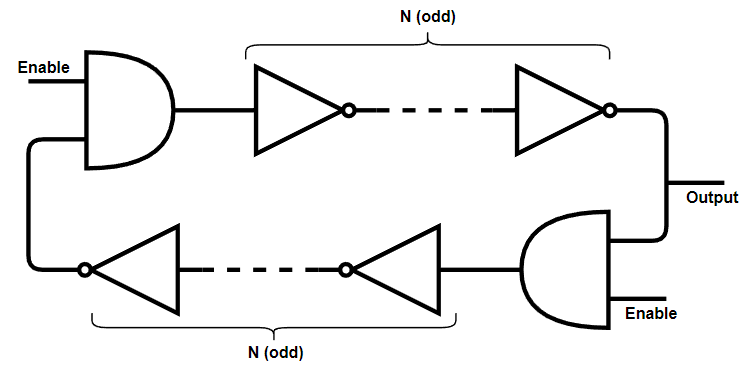
\includegraphics[width=0.55\linewidth]{images/tero_structure.png}
   \caption{\label{fig:cell_diagram}TERO cell logical representation}
\end{figure}

The structure of the \acrshort{tero} cell (represented in figure~\ref{fig:cell_diagram}) is related to the \acrshort{sr-latch} but where the \textit{set} and \textit{reset} inputs are used simultaneously (the \textit{enable} signal on the diagram). The two opposite AND gates serve as the entry point for the signals when the cell is enabled, and an equal and odd number of NOT gates on each branch create a delay inside the loop. The initial state (when \textit{enable} is low) is stable, as represented in figure~\ref{fig:ter_cell_states}(a).\\

Once \textit{enable} is set to high, this circuit becomes an oscillator with two signals propagating inside the loop, which toggles the output signal. Due to the imperfect nature of any real \acrshort{ic}, one signal will eventually catch up with the other, they will cancel each other, stopping the oscillation and reaching one of the two stable states, represented in figure~\ref{fig:ter_cell_states}(b). The final state depends on which signal catches the other. At this point, the cell will stay in this state until the \textit{enable} signal falls, which will reset the cell to the initial state through the AND gates. The number of NOT gates on each branch (noted N) is used as a parameter to choose the length of the propagation path inside the cell but needs to remain odd.\\

\begin{figure}[H]
   \begin{minipage}[b]{0.50\linewidth} 
        \centering
        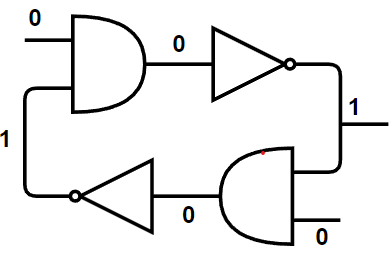
\includegraphics[width=0.6\linewidth]{images/tero_init_state.png}
        \subcaption{Initial state}
   \end{minipage}\hfill
   \begin{minipage}[b]{0.50\linewidth}   
        \centering
        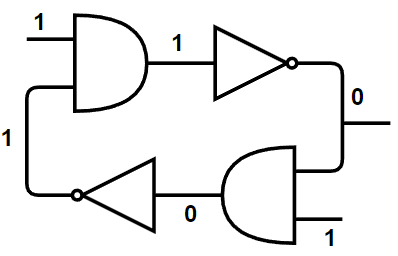
\includegraphics[width=0.6\linewidth]{images/tero_final_state.png}
        \subcaption{Final state}
   \end{minipage}
   \caption{\label{fig:ter_cell_states}\acrshort{tero} cell states (N=1)}
\end{figure}

The effect of the random defect of the \acrshort{ic} on this circuit can be observed in two ways: the final state reached after stabilisation and the number of oscillations reached before this stabilisation. These two properties can be used to generate bits from this structure.


\section{Response generation}
\label{sec:design_generation}


The PUF needs to generate a sequence of bits from the \acrshort{tero} cells, using either the final state or the final number of oscillations. To do so, the simplest method could consist of using the final state of the cell directly as the bit response since it has only two possible states. This is represented in the figure~\ref{fig:generative_meth_1}.\\

This has the advantage of being very simple to implement. However, the issue with this technique is that the cells need to be perfectly reliable or the bits would not be stable. It has been shown in~\cite{bossuet_puf_2014, marchand_implementation_2017} that some cells take much more time to stabilise, to the point where they can be considered as "unstable" and will produce an unreliable bit. An additional drawback is that the number of bits that can be generated is equal to the number of \acrshort{tero} cells. Therefore, the resource usage for this method scales linearly with the size of the response. \\



\begin{figure}[H]
   \begin{minipage}[b]{0.47\linewidth} 
        \centering
        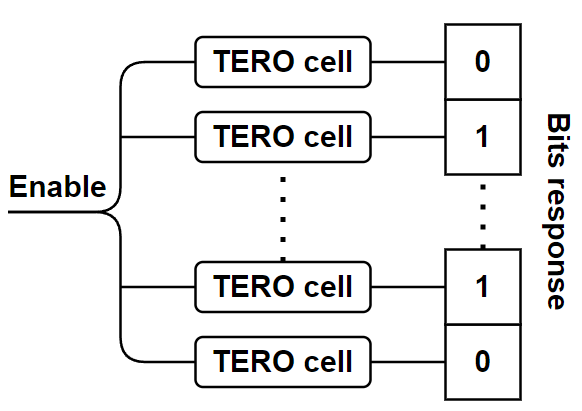
\includegraphics[width=\linewidth]{images/generative_meth_1.png}
        \subcaption{Direct\label{fig:generative_meth_1}}
   \end{minipage}\hfill
   \begin{minipage}[b]{0.53\linewidth}   
        \centering
        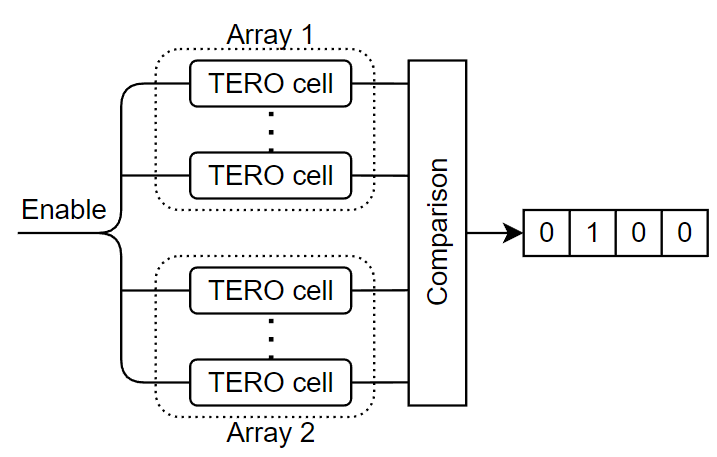
\includegraphics[width=\linewidth]{images/generative_meth_2.png}
        \subcaption{Comparison\label{fig:generative_meth_2}}
   \end{minipage}
   \caption{Bit generation method}
\end{figure}


Another approach (represented in figure~\ref{fig:generative_meth_2}) is to compare the number of oscillations of two cells after stabilisation. A '1' is generated if the first cell has a higher number of oscillations, and a '0' is generated otherwise. This is the method used by~\cite{de_weerdt_implementation_2021}.\\

This method is less sensitive to the cell's exact number of oscillations in terms of the reliability of the response as long as the number of oscillations of the different cells is clearly spread. By splitting K cells into two arrays for the comparison, the number of bits that can be generated is equal to $\left ( \frac{K}{2}\right )^2$. This scales quadratically with the size of the response, which is better than the first method. One can notice that equality between the two cells will always generate a '0' in this method. This could degrade the uniformity of the response if too many equalities occur and this is something that will need to be tested once the \acrshort{puf} is implemented.\\


A third design, the gray coding response generation, used in~\cite{marchand_implementation_2017}, is to subtract the number of oscillations of two cells, apply a Gray coding on this value then select specific bits from this code to create a part of the response. 
This has the disadvantage that the bits need to be analysed to determine which ones are the more stable in order to select them to generate a chip ID that is reliable. This also adds additional elements to the design compared to the second method.

\begin{figure}[H]
    \centering
    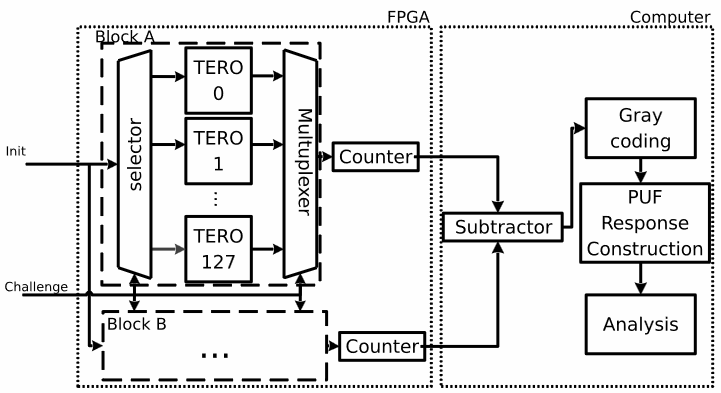
\includegraphics[width=0.75\linewidth]{images/tero_gray_coding.png}
    \caption{Gray coding response generation (figure from~\cite{marchand_implementation_2017})}
    \label{fig:generative_meth_3}
\end{figure}

The second method is chosen because it has a small footprint while producing a response with good reliability. Furthermore, it also ensures higher compatibility with the implementation of~\cite{de_weerdt_implementation_2021}.\\

To maximise the size of the response, each cell should be compared to every cell of the opposite array. Instead of storing all the possible combinations in memory,~\cite{de_weerdt_implementation_2021} has proposed to use a \acrfull{lsfr} circuit to compute them as needed. Indeed, a such circuit will cycle through the entire possible $2^{N} -1$ values exactly once before returning to the initial state (where N is the size of the register). The first half bits of the \acrshort{lsfr} can be used as a selection for the first array, and the remaining bits for the second array.

This way, all the possible combinations are covered except the 0-0 one because the state with only '0' is a forbidden state (the \acrshort{lsfr} would stay in this state forever), reducing the size of the response bit one. For a large enough number of cells, this impact will become negligible. Moreover, this implementation takes very little hardware resources and scale better than storing all the combination in memory. For those reasons, this \acrshort{lsfr} will also be used in this implementation. The new size of the \acrshort{puf} response is therefore equal to $\left ( \frac{K}{2}\right )^2 -1$.

\begin{figure}[H]
    \centering
    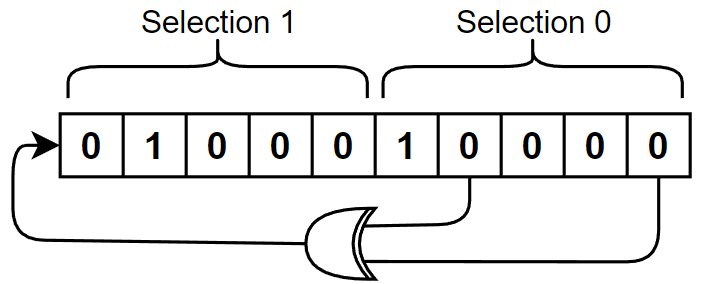
\includegraphics[width=0.5\linewidth]{images/LSFR.png}
    \caption{10-bits \acrshort{lsfr}}
    \label{fig:LSFR}
\end{figure}

\section{TERO-PUF operation}
\label{sec:design_operation}

We can now fully describe the operation of our \acrshort{teropuf}: the \acrshort{tero} cells are composed of 2 AND gates and $2\times N$ NOT gates (N is odd). K cells are split into two arrays (K need to be even). Each possible pair (except the '0-0' one) is selected in turn using an \acrshort{lsfr}. For each pair, the two selected cells are enabled at the same time along with a reference counter connected to the clock, and the number of oscillations is recorded. Once the reference counter reaches the number of clock cycles corresponding to the desired acquisition time, the number of oscillations is compared and one bit of the response is generated. Then the cells and the reference counter are disabled, which reset their state, and the \acrshort{lsfr} is shifted to generate the next combination to be selected. $\left ( \frac{K}{2}\right )^2 -1$ bits are generated in this way. The usage of the reference counter imposes that the acquisition time can only be a multiple of the clock period ($\frac{1}{f}$)\\


\begin{figure}[H]
    \centering
    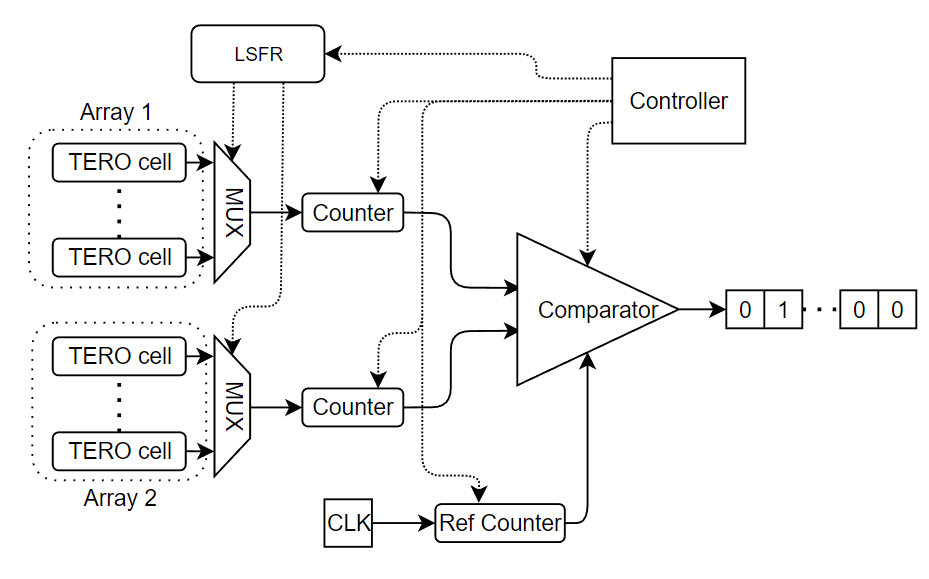
\includegraphics[width=1\linewidth]{images/puf_block.png}
    \caption{\acrshort{teropuf} block diagram}
    \label{fig:generative_sum}
\end{figure}




%FOCUS HERE !

%REF: Design and caracterization of TERO-PUF and SRAMs

%Only the universal concepts, put implementation in result

%Shows the difference (> contribution) from the other study on TERO-PUF

\chapter{FPGA implementations and characterisation}
\label{ch:impl&chara}

In this chapter, two \acrshort{vhdl} implementations for the ARTIX-7 \acrshort{fpga} will be proposed, based on the concept presented in the previous chapter. The feature developed for demonstrative purposes will also be presented more in-depth. Finally, a report of the \acrshort{fpga} resources usage of the BASYS-3 board that will be used for testing in the next section will be provided.\\

\section{Implementation}
\label{sec:impl}

In this section, we will first study the constraints that need to be respected to apply the proposed design to an \acrshort{fpga} implementation for ARTIX-7. This will add restrictions to the design and will lead us to two possible implementations.

Artix-7 \acrfull{clb} a made up of two slice of 4 \acrshort{lut}s, highlighted on green in figure~\ref{fig:clb_routing} and an inter-clb routing block (magenta) for the interface with the global routing of the \acrshort{fpge}. The internal routing can be programmed between \acrshort{lut}s as well.


\begin{figure}[H]
    \centering 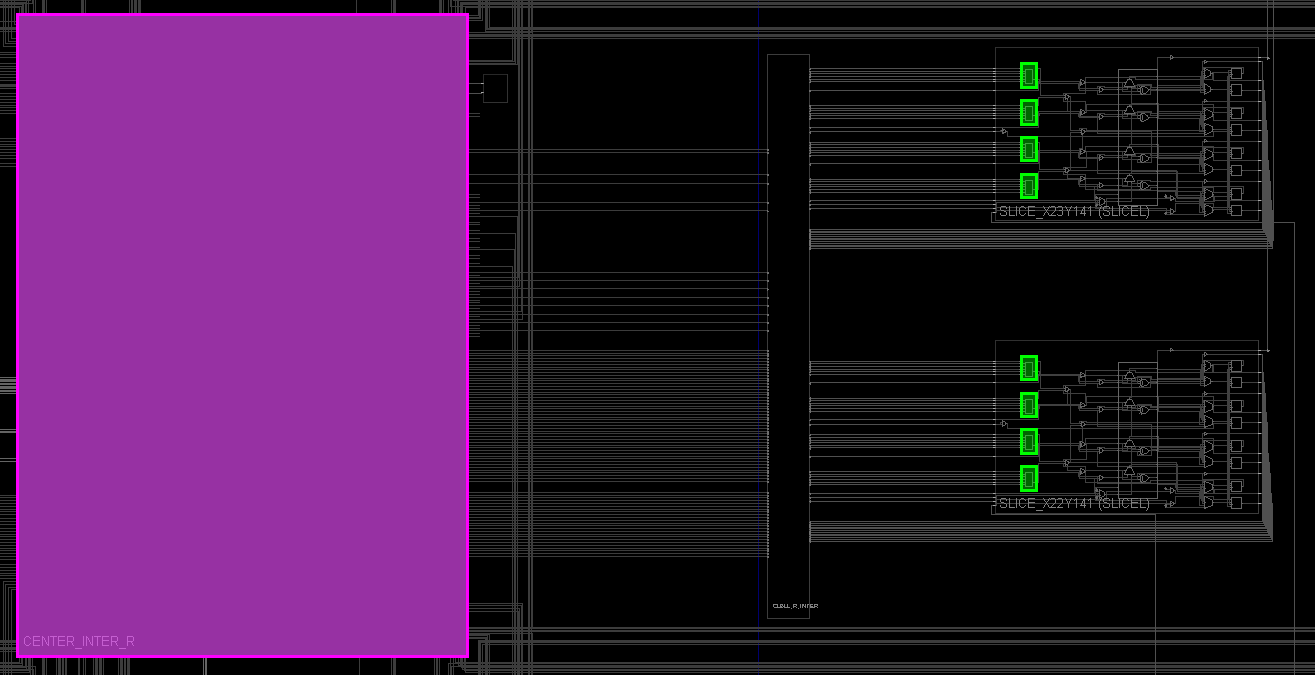
\includegraphics[width=0.9\linewidth]{images/clb_routing.png}
    \caption{Artix-7 CLB}
    \label{fig:clb_routing}
\end{figure}


\subsection{Constraints}
\label{subsec:impl_constraints}

The behaviour of the cells is very sensitive, not only to random defects in the \acrshort{ic} but to any difference both in terms of implementation (length of the loop, placement, etc...) and external factors (ageing, temperature, voltage). Therefore, to ensure that the \acrshort{puf} response is generated from the random defects with as little bias, the cell implementation should be as identical as possible. To achieve this, the \acrfull{xdc} are used to manually specify some properties of specific parts of the design.\\

By default, Vivado will try to optimise the design without changing the logical behaviour of the circuit. However, since the cell's exact behaviour is based on random defects, it can not be correctly interpreted by Vivado and any optimisation will most likely break the design. Therefore, the first constraint used is the \textbf{DONT\_TOUCH} to tell Vivado to not try to optimise the design of the cells so that it remains untouched.\\

Furthermore, the slices used to implement the cells should be the same type. On the ARTIX-7, there are two main types of slice: SLICEL (only for combinatorial functions) and SLICEM (can additionally implement memory features). There is a higher number of SLICEL available and the \acrshort{tero} cells do not need any memory functionalities. For this reason, only SLICEL are used for the PUF implementation. This is archived using \textbf{LOC} constraints.\\


The routing of the internal loop between the LUTs should also be identical. To simplify the routing management, constraining the cells to only one \acrshort{clb} could ensure that the internal loop does not need to use global routing and can stay inside the \acrshort{clb}. The \textbf{BEL} is used to fix the exact LUT used for an element and \textbf{RLOC} to place elements in slices that are next to each other. It is also possible to assign each input to a specific pin of the LUTs using \textbf{LOCK\_PINS}, to ensure an identical internal path for all the cells.\\
More details on how these \acrshort{xdc} constraints are used can be found in appendix~\ref{appendix:constraints}.\\

\subsection{Cell size}
\label{subsec:imple_cell_size}

From the routing constraints discussed previously, we know that it is preferable to use only one \acrshort{clb} to implement our cell because it removes the need for inter-\acrshort{clb} routing. On ARTIX-7, \acrshort{clb} contain two slices of 4 \acrshort{lut}s each. The design of the \acrshort{tero} cells imposes to have 2 AND gates and $2 N$ NOT gates with N being odd. This restricts our choice of the number of NOT gates to $N = \{1, 3\}$, which correspond to 4 and 8 LUTs respectively. Both cases are studied in parallel and their schematics are shown in figure~\ref{fig:tero_cell_4_&_8_diagram}. The first one will be noted TERO-4 and the second one TERO-8, due to their LUT usage.

\begin{figure}[H]
   \begin{minipage}[b]{\linewidth} 
        \centering
        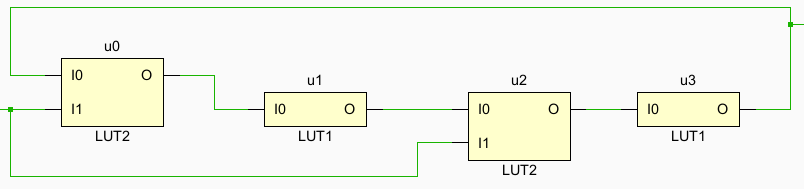
\includegraphics[width=\linewidth]{images/tero_4_schematic.png}
        \subcaption{TERO-4 (N=1)}
   \end{minipage}
   \begin{minipage}[b]{\linewidth}   
        \centering
        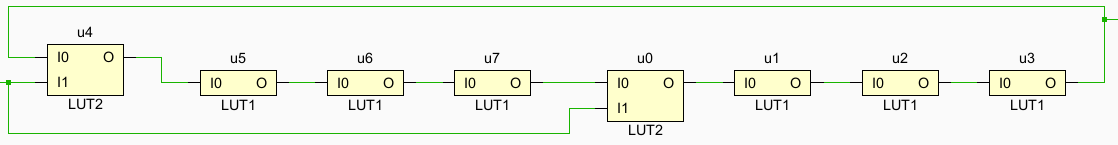
\includegraphics[width=\linewidth]{images/tero_8_schematic.png}
        \subcaption{TERO-8 (N=3)}
   \end{minipage}
   \caption{\label{fig:tero_cell_4_&_8_diagram}\acrshort{tero} cells schematics}
\end{figure}

Figure~\ref{fig:tero_8_cell_routing} represent a TERO-8 cell with the eight \acrshort{lut} in orange,  one of the internal signal is highlighted in white and the reset in green.

\begin{figure}[H]
    \centering 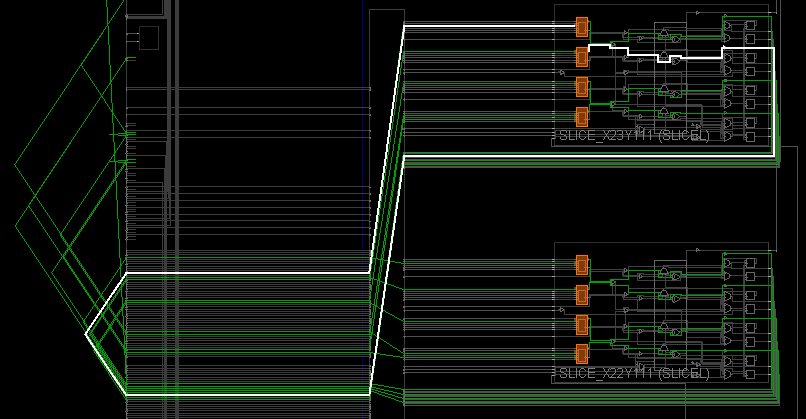
\includegraphics[width=0.9\linewidth]{images/cell_routing.png}
    \caption{TERO-8 cell routing}
    \label{fig:tero_8_cell_routing}
\end{figure}

\subsection{Number of cells}
\label{subsec:impl_number_of_cell}




\begin{minipage}[b]{0.55\linewidth} 
The initial discussion about the method to generate the response (section~\ref{sec:design_generation}) provided us with a relation between the number of cells and the response size:  $\left ( \frac{K}{2}\right )^2 -1$. The size of the PUF response needs to be high enough to be able to study their statistical properties. $2\times32$ cells are chosen here, which gives a response of 1023 bits.\\

For the implementation using TERO-8 cells, the number of slices needed is doubled but it is still possible to contain the entire implementation in a single die of the BASYS-3 board used for testing. The figure~\ref{fig:tero_8_slice_usage_overview} represents the TERO-8 cells regrouped together, with one cell (2 slices) highlighted in green. This left plenty of areas to implement other functionalities in the same device.
\end{minipage}\hfill
\begin{minipage}[b]{0.32\linewidth}   
    \centering
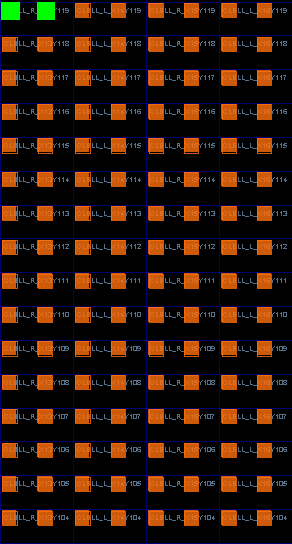
\includegraphics[width=\linewidth]{images/tero_8_array_CLB.png}
\captionof{figure}{Slices usage of TERO-8 cells arrays\label{fig:tero_8_slice_usage_overview}}
\end{minipage}

\section{Demonstrative features}
\label{sec:demon_feature}

To provide a demonstration of a security procedure using the \acrshort{tero}, some additional features are embedded in the implementation: a \acrfull{bch} decoder for error correction and a \acrshort{sha}-256 hashing function\\

\subsection{BCH decoder}
\label{subsec:demon_feature_bch}

\acrshort{ecc} are good options to improve the reliability of the response. Commonly used in applications such as satellite communication, CD-player or USB flash drive, the \acrshort{bch} code operates using helper data (called syndrome) to correct up to a certain number of random errors. It is represented using 3 parameters $BCH(N, K)$: $N$ is the size of encoded data length and $K$ is the message length. This also fixes the maximal number of errors that can be successfully corrected $T$, as well as the syndrome's size $N - K$ \cite{freudenberger_reduced_2021}.\\

The syndrome is computed beforehand from the reference response (during the provision step) and can be either stored on the device or transmitted when needed. The syndrome can be fully revealed since it does not contain any information useful to predict the original response. During the evaluation step, the response of the PUF is checked with the help of the syndrome, and as long as the number of errors is lower than $T$, it can correct them.\\

In the implementation of \cite{de_weerdt_implementation_2021}, an \acrshort{bch} decoder was added in the FPGA design, and the syndrome was computed externally (using Matlab) and then send to the device when needed. The same \acrshort{bch} implementation is used in this thesis. The parameter has been set to $BCH(255, 171)$, therefore only the first 171 bits of the PUF response are considered. This corresponds to $T=11$ correctable errors and a syndrome of 84 bits. This is enough to study the improvement in the reliability while having a moderate area usage overhead as we will see in chapter~\ref{ch:result}.\\

\begin{figure}[H]
    \centering 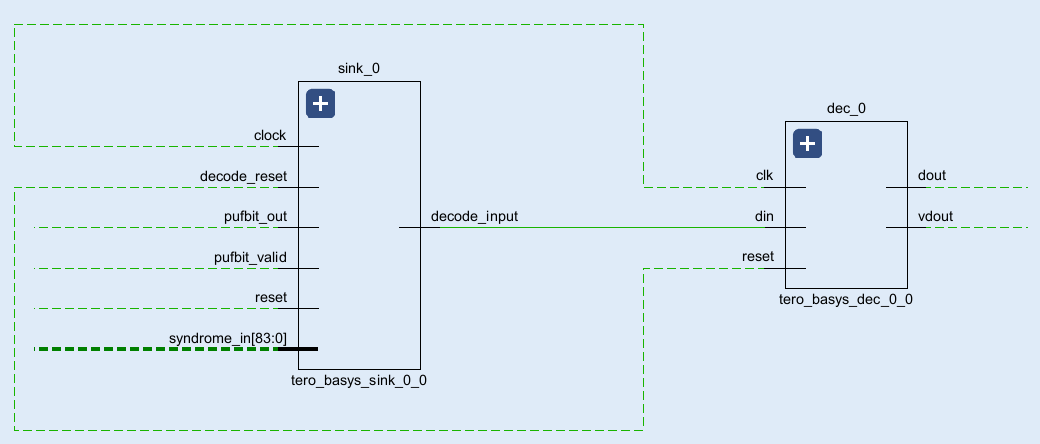
\includegraphics[width=\linewidth]{images/bch_schematic.png}
    \caption{BCH(255, 171) schematic}
    \label{fig:bch_schematic}
\end{figure}

One can notice that due to the way the cell combinations are produced by the \acrshort{lsfr}, taking only the first bits of the responses will lead to a non-uniform usage of the cells for those retained bits. This is discussed in the appendix~\ref{appendix:lsfr} where we conclude that this does not have a significant impact on the results found in the next section.



\subsection{SHA-256}
\label{subsec:demon_feature_sha}

A hashing function can be useful to transform the \acrshort{puf}'s response into a usable key for security applications. Since one goal of this study was to improve the demonstration part of the framework, it has been chosen to implement this \acrshort{sha}-256 algorithm in the \acrshort{fpga} itself.\\

There are already \acrshort{vhdl} implementations available with open-source licenses online. Therefore, it had been chosen not to re-implement those well-defined operations and to use one of these. The implementation we selected is from the GitHub repository of the user "\textbf{batiati}" \cite{batiati_vhdl_2021}. The author made available two implementations: one that operates on a single chunk of 512 bits, and the second that operates as a pipeline. We will only need to hash a single key at a time so the first implementation is sufficient.\\

The \acrshort{sha}-256 hashing operate on a block of 512 bits, that need to be padded from the original input as explained in ~\cite{technology_secure_2015}. First, the input need to be split into blocks of 447 bits maximum. To those blocks, a single \textbf{'1'} is added, and then we pad with \textbf{'0'} until the block reaches 448 bits. Finally, the 64 remaining bits are the length of the initial input (between 0 and 447) in binary form.

In our case, the input is the response of the \acrshort{bch} decoder. This always has the same size (171 bits) and fits into a single block. The corresponding padded block is represented in table~\ref{tab:sha256_padding}.\\

\begin{table}[H]
    \centering
    \begin{tabular}{|c|c|c|c|}
        \hline
        Input & Single \textbf{1} & \textbf{0} padding & Input size (64 bits)\\
        \hline
        171 bits & 1 bit & 276 bits & 64 bits\\
        \hline
        \textit{PUF after BCH} & \textbf{1} & \textbf{00..00} & \textbf{0000 ... 1010 1011} \\
        \hline
    \end{tabular}
    \caption{512 block padding for \acrshort{sha}-256}
    \label{tab:sha256_padding}
\end{table}

This gives us the complete \acrshort{sha}-256 block represented in figure~\ref{fig:sha_schematic} with first the padding block receiving bit from the \acrshort{bch} decoder, followed by the \acrshort{sha} block. It has been validated it using test vectors from the \acrfull{nist}~\cite{computer_security_division_example_2016} before adding it to the rest of our implementation.\\

\begin{figure}[H]
    \centering
    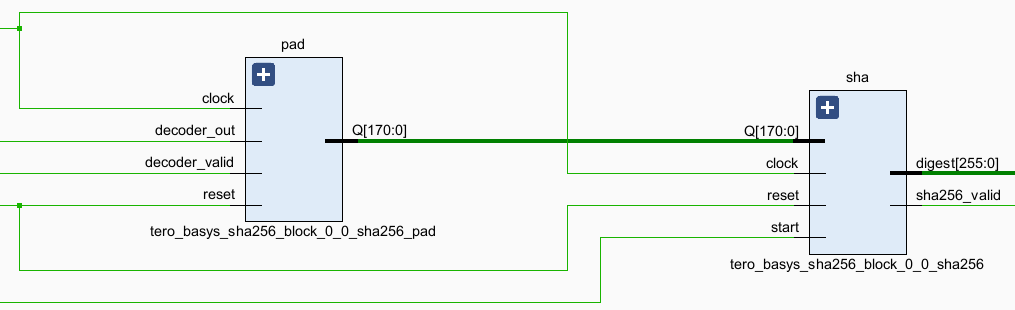
\includegraphics[width=\linewidth]{images/sha256_schematic.png}
    \caption{\acrshort{sha}-256 block schematic}
    \label{fig:sha_schematic}
\end{figure}

\section{FPGA usage}
\label{sec:fpga_usage}

We have now described all elements of our TERO PUF implementations for the ARTIX-7. The first step to characterise it is to analyse the resources used on the boards.

\subsection{Area}
\label{subsec:fpga_usage_area}

The total area usage of the implementation on a Basys-3 board can be seen in figure~\ref{fig:overview_area_usage}. The slices used for \acrshort{tero} cells are coloured orange because they have a fixed location, while the rest of the used area is light blue.

\begin{figure}[H]
    \centering
    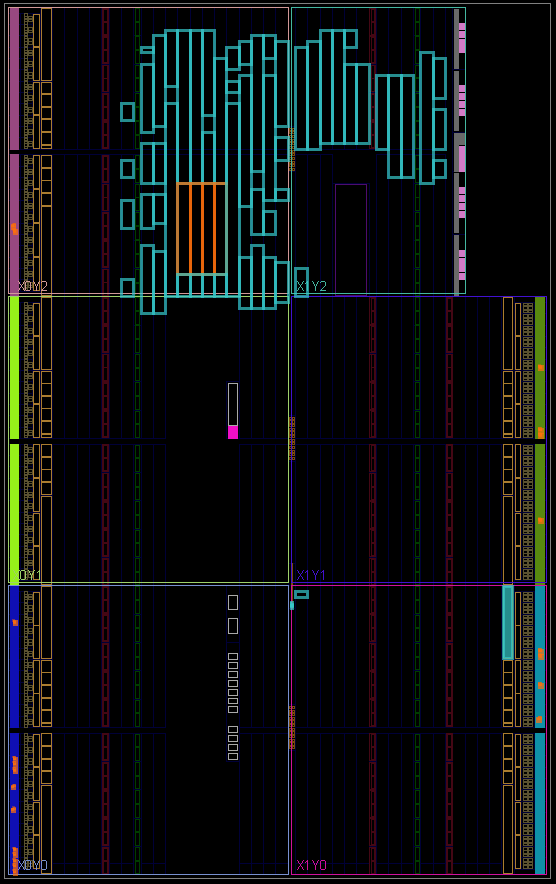
\includegraphics[width=0.65\linewidth]{images/overview_area_usage.png}
    \caption{Total area usage}
    \label{fig:overview_area_usage}
\end{figure}



The individual blocks can also be highlighted to show the placement made by Vivado. This is done on figure~\ref{fig:fpga_area_usage_detailled} for the \acrshort{puf} block (containing the cells and the elements required to generate the response), the control and \acrfull{uart} block, the \acrshort{bch} decoder and the \acrshort{sha}-256.

\begin{figure}[H]
   \begin{minipage}[b]{0.5\linewidth} 
        \centering
        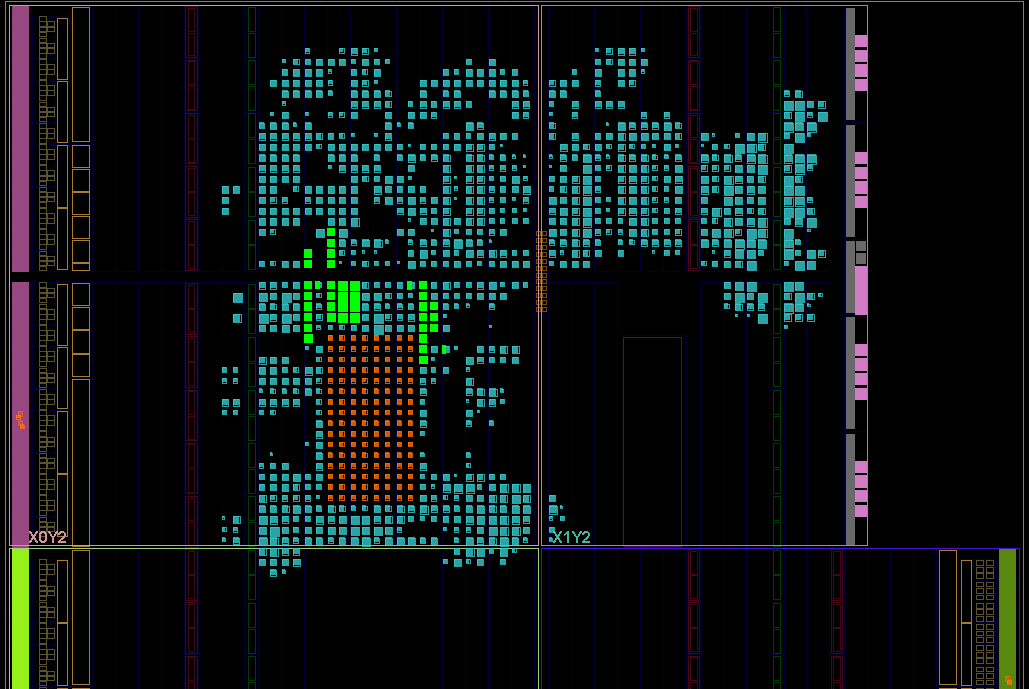
\includegraphics[width=\linewidth]{images/tero_block_area_usage.png}
        \subcaption{\acrshort{puf} block}
   \end{minipage}\hfill
   \begin{minipage}[b]{0.5\linewidth}   
        \centering
        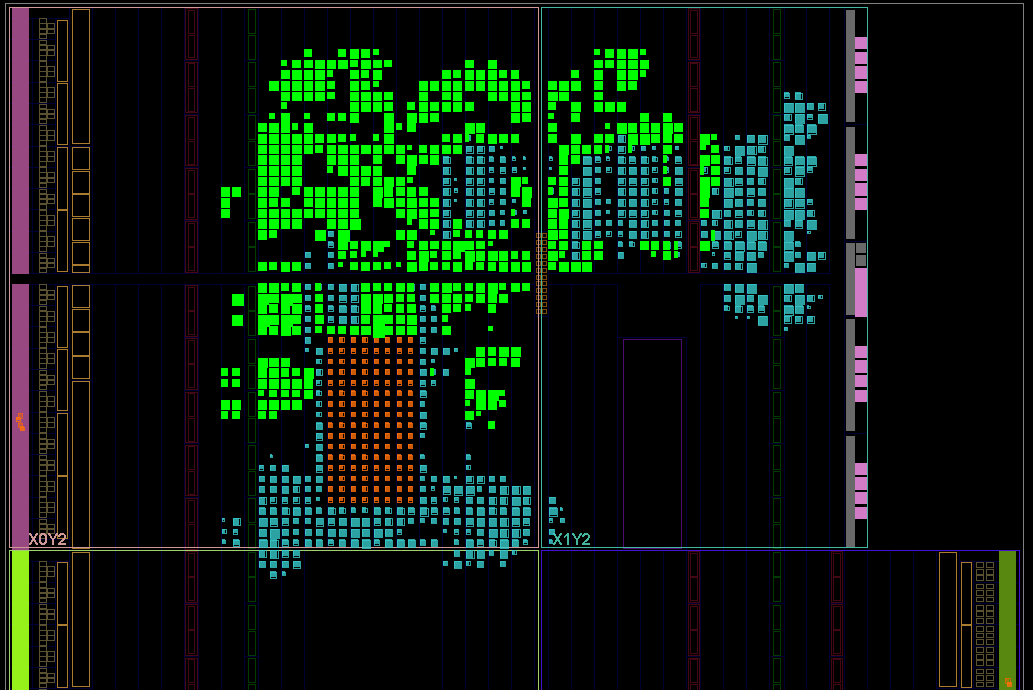
\includegraphics[width=\linewidth]{images/control_and_interface_area_usage.png}
        \subcaption{Control \& \acrshort{uart}}
   \end{minipage}
   \begin{minipage}[b]{0.5\linewidth} 
        \centering
        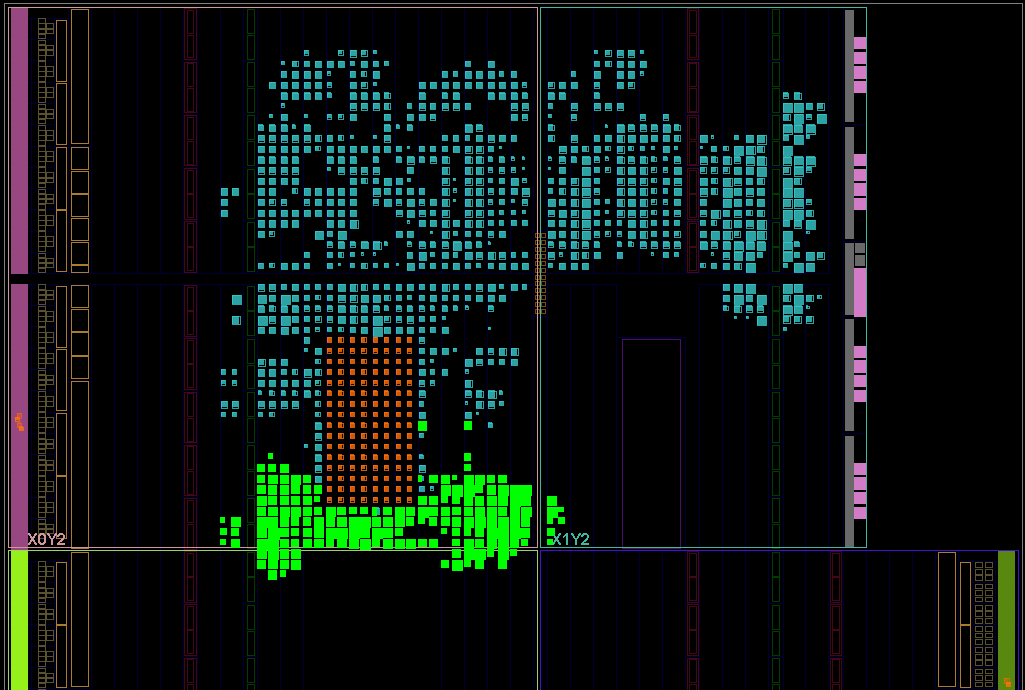
\includegraphics[width=\linewidth]{images/decoder_area_usage.png}
        \subcaption{\acrshort{bch} decoder}
   \end{minipage}\hfill
   \begin{minipage}[b]{0.5\linewidth}   
        \centering
        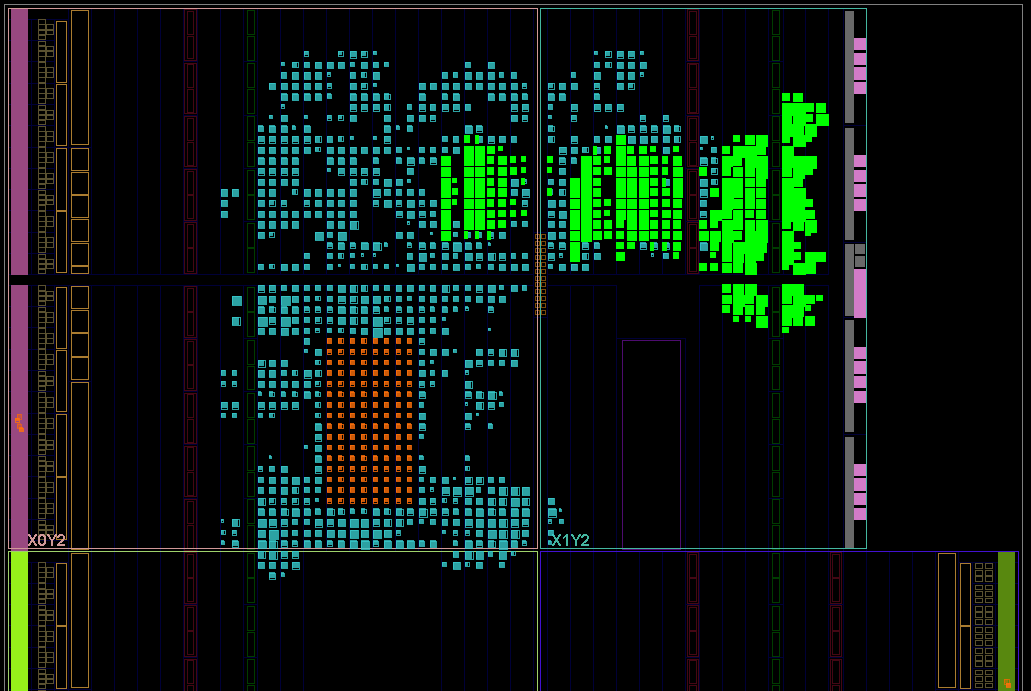
\includegraphics[width=\linewidth]{images/sha256_area_usage.png}
        \subcaption{\acrshort{sha}-256}
   \end{minipage}
   \caption{\label{fig:fpga_area_usage_detailled}Basys-3 usage per block}
\end{figure}

The primitive statistic for each part of the implementation is reported on the tables~\ref{tab:tero_4_fpga_area_usage} and \ref{tab:tero_8_fpga_area_usage}, as well as the total usage reported by Vivado.

\begin{table}[H]
    \centering
    \begin{tabular}{|l|c|c|}
         \hline
         \textbf{Primitive statistic} & \textbf{LUTs} & \textbf{Flop latches} \\
         \hline
         TERO-4 \acrshort{puf} Block & 428 | 11\% & 162 | 5\% \\
         \hline
         \acrshort{bch} decoder & 797 | 20\% & 981 | 29\%\\
         \hline
         \acrshort{sha}-256 & 895 | 23\% & 950 | 28\%\\
         \hline
         Control \& \acrshort{uart} & 1792 | 46\% & 1308 | 38\%\\       
         \hline
         Total & 3912 & 3401\\
         \hline
    \end{tabular}
    \caption{TERO-4 \acrshort{fpga} resources usage}
    \label{tab:tero_4_fpga_area_usage}
\end{table}


\begin{table}[H]
    \centering
    \begin{tabular}{|l|c|c|}
         \hline
         \textbf{Primitive statistic} & \textbf{LUTs} & \textbf{Flop latches} \\
         \hline
         TERO-8 \acrshort{puf} Block & 684 | 16\% & 162 | 5\% \\
         \hline
         \acrshort{bch} decoder & 797 | 19\% & 981 | 29\%\\
         \hline
         \acrshort{sha}-256 & 895 | 21\% & 950 | 28\%\\
         \hline
         Control \& \acrshort{uart} & 1792 | 43\% & 1308 | 38\%\\       
         \hline
         Total & 4168 & 3353\\
         \hline
    \end{tabular}
    \caption{TERO-8 \acrshort{fpga} resources usage}
    \label{tab:tero_8_fpga_area_usage}
\end{table}

The TERO-8 \acrshort{puf} block requires more resources than the TERO-4 one, which makes sense since the TERO-8 cells need twice as many slices then the TERO-4 ones. In both cases, it is the less significant part of the implementations and the control \& \acrshort{uart} takes most of the space.

\subsection{Power consumption}
\label{subsec:fpga_usage_pwr}

\begin{figure}[H]
    \centering
    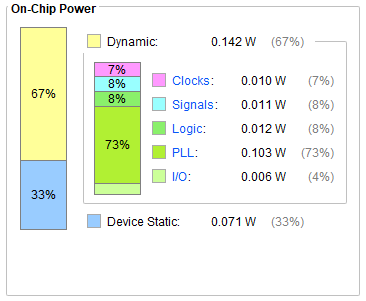
\includegraphics[width=0.7\linewidth]{images/power_usage.png}
    \caption{Power report for TERO-8}
    \label{fig:tero_8_power_usage}
\end{figure}

The power report from Vivado\ref{fig:tero_8_power_usage} indicate an estimated 0.142W of dynamic and an additional 0.071W for the static part such that the total estimated power consumption is 0.213W. We can see that the higher contribution (73\%) is the \acrfull{pll} and that the remaining parts only consume 0.039W (27\%).




%FOCUS HERE !

%TERO-PUF: FPGA implementation and caracterisation

%Implementation (this experiment specific concept also !) > features > PPE > PUF

%Shows the difference (> contribution) from the other study on TERO-PUF

%More on the experimental setup (specify ambiant temp, voltage, ... -> futur work)

%FPGA Usage (PPE)

\chapter{PUF results and demonstration}
\label{ch:result}

To fully characterise the \acrshort{puf} performance of the two implementations, the following aspects are studied:

\begin{itemize}
    \item The oscillations of the \acrshort{tero} cells over time.
    \item The intra-device metrics (uniformity and reliability) for different acquisition times on a single device.
    \item The inter-device metrics (average uniformity and reliability, uniqueness and bit-aliasing) are computed from the result of 33 devices for a chosen acquisition time.
    \item The impact of the \acrfull{ecc}.
\end{itemize}

Furthermore, the performance found will be compared to other existing \acrshort{teropuf} implementations, followed by a description of the demonstration.\\

All tests are run on Basys-3 with the main clock frequency being 100 MHz. Each data point is averaged over 10 000 samples. The tests were done with an ambient temperature around 20\textdegree C and nominal voltage.\\

The interface between the FPGA and the computer is done via UART and a custom Python module described in appendix~\ref{appendix:python_mod}

\section{Cells behaviour and equalities}

The value of the counter of each cell is directly sent via \acrshort{uart} once the acquisition time is reached, instead of being compared to generate the \acrshort{puf} response. The range of acquisition time to evaluate is chosen from $0.01\mu s$ to $2\mu s$. The expected behaviour is to initially have several oscillations at the beginning, then at some point, reach stability and remain constant.

\subsection{Oscillations over time}
\subsubsection*{TERO-4}

The 64 TERO-4 cell's oscillations are displayed in figure~\ref{fig:tero_4_oscillation_vs_time}. The cells stabilise within a single clock cycle ($0.01\mu s$) with a final number of oscillations below 20, except for one cell that only stabilises around $0.4\mu s$ after 160 oscillations.

\begin{figure}[H]
   \begin{minipage}[b]{\linewidth} 
        \centering
        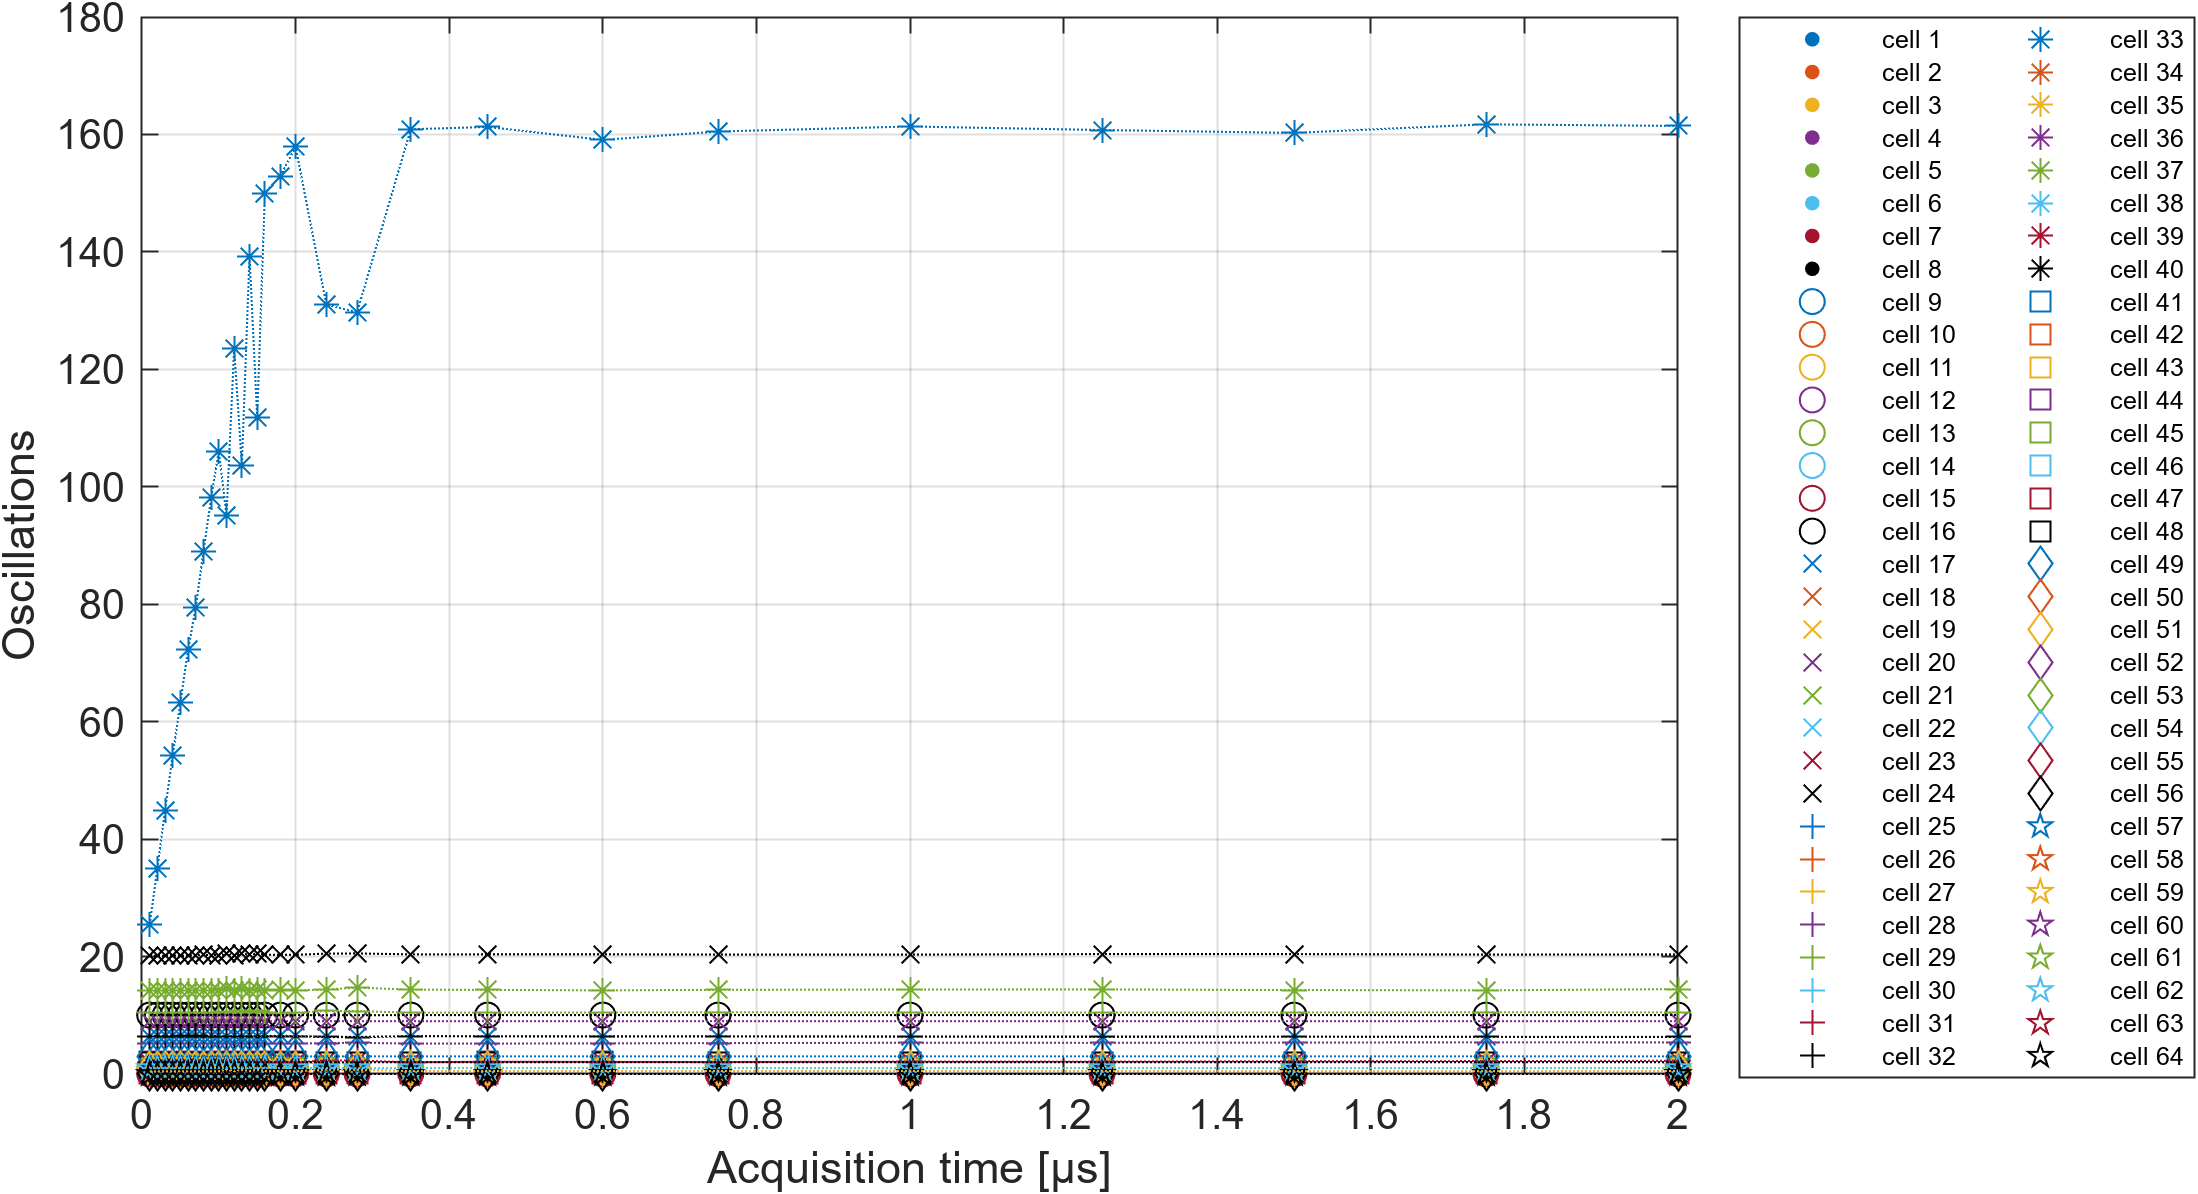
\includegraphics[width=\linewidth]{images/tero_4_oscillations_vs_time.png}
        \subcaption{Full\label{fig:tero_4_oscillation_vs_time_full}}
   \end{minipage}
   \begin{minipage}[b]{\linewidth}   
        \centering
        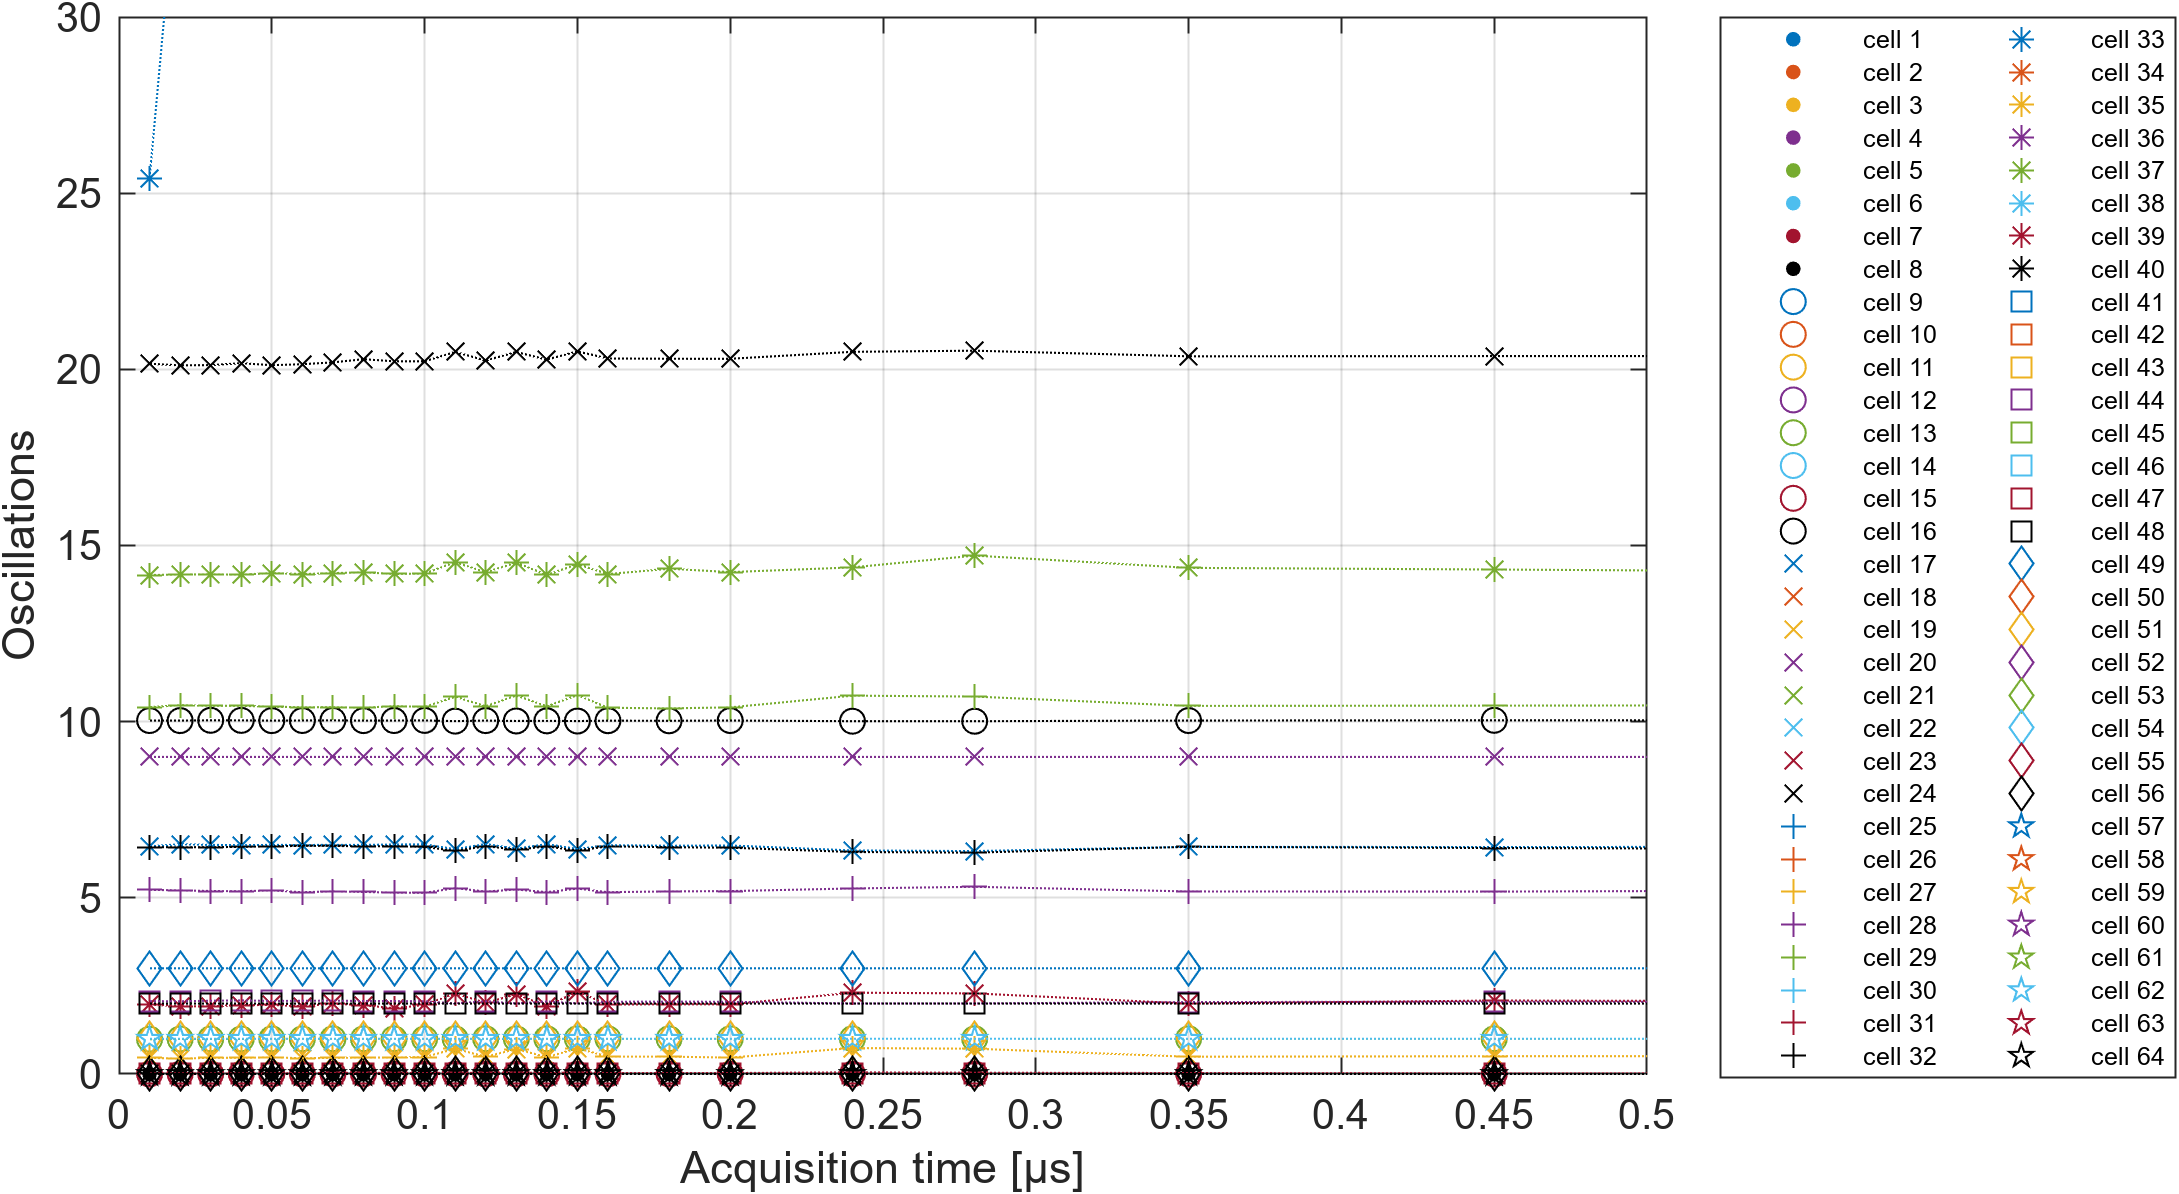
\includegraphics[width=\linewidth]{images/tero_4_oscillations_vs_time_zoomed.png}
        \subcaption{Zoomed\label{fig:tero_4_oscillation_vs_time_zoomed}}
   \end{minipage}
   \caption{TERO-4 cells oscillations over acquisition time\label{fig:tero_4_oscillation_vs_time}}
\end{figure}

\subsubsection*{TERO-8}

The figure~\ref{fig:tero_8_oscillation_vs_time} represents the oscillation of the 64 TERO-8 cells. The stabilisation time is mostly below $0.5 \mu s$. Four cells seem to never really stabilise before $2\mu s$. The final number of oscillations of the stable cells is spread up to 200.\\

\begin{figure}[H]
   \begin{minipage}[b]{\linewidth} 
        \centering
        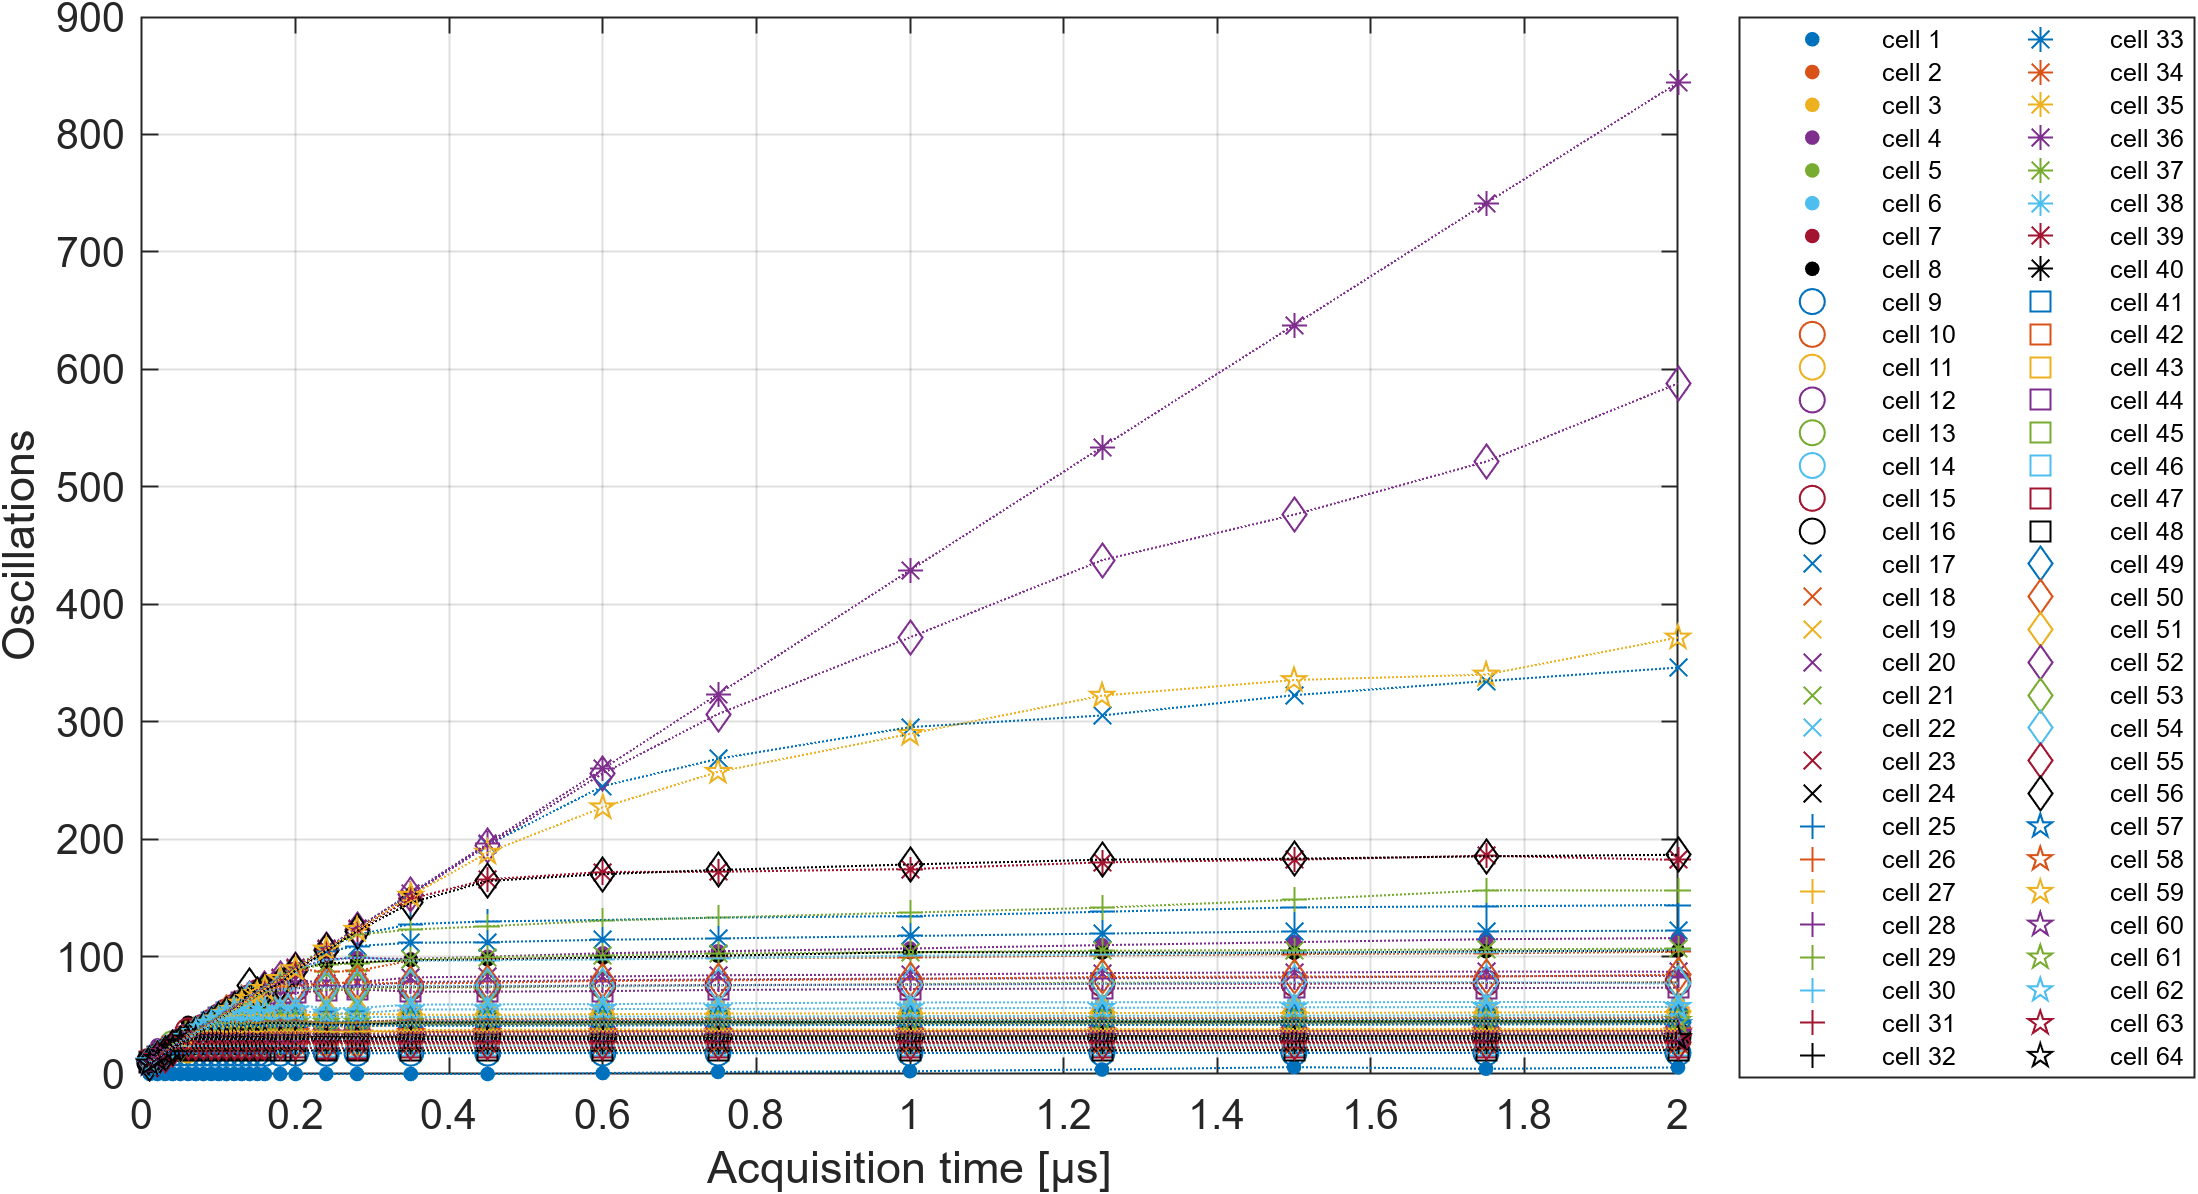
\includegraphics[width=\linewidth]{images/tero_8_oscillations_vs_time.png}
        \subcaption{Full\label{fig:tero_8_oscillation_vs_time_full}}
   \end{minipage}
   \begin{minipage}[b]{\linewidth}   
        \centering
        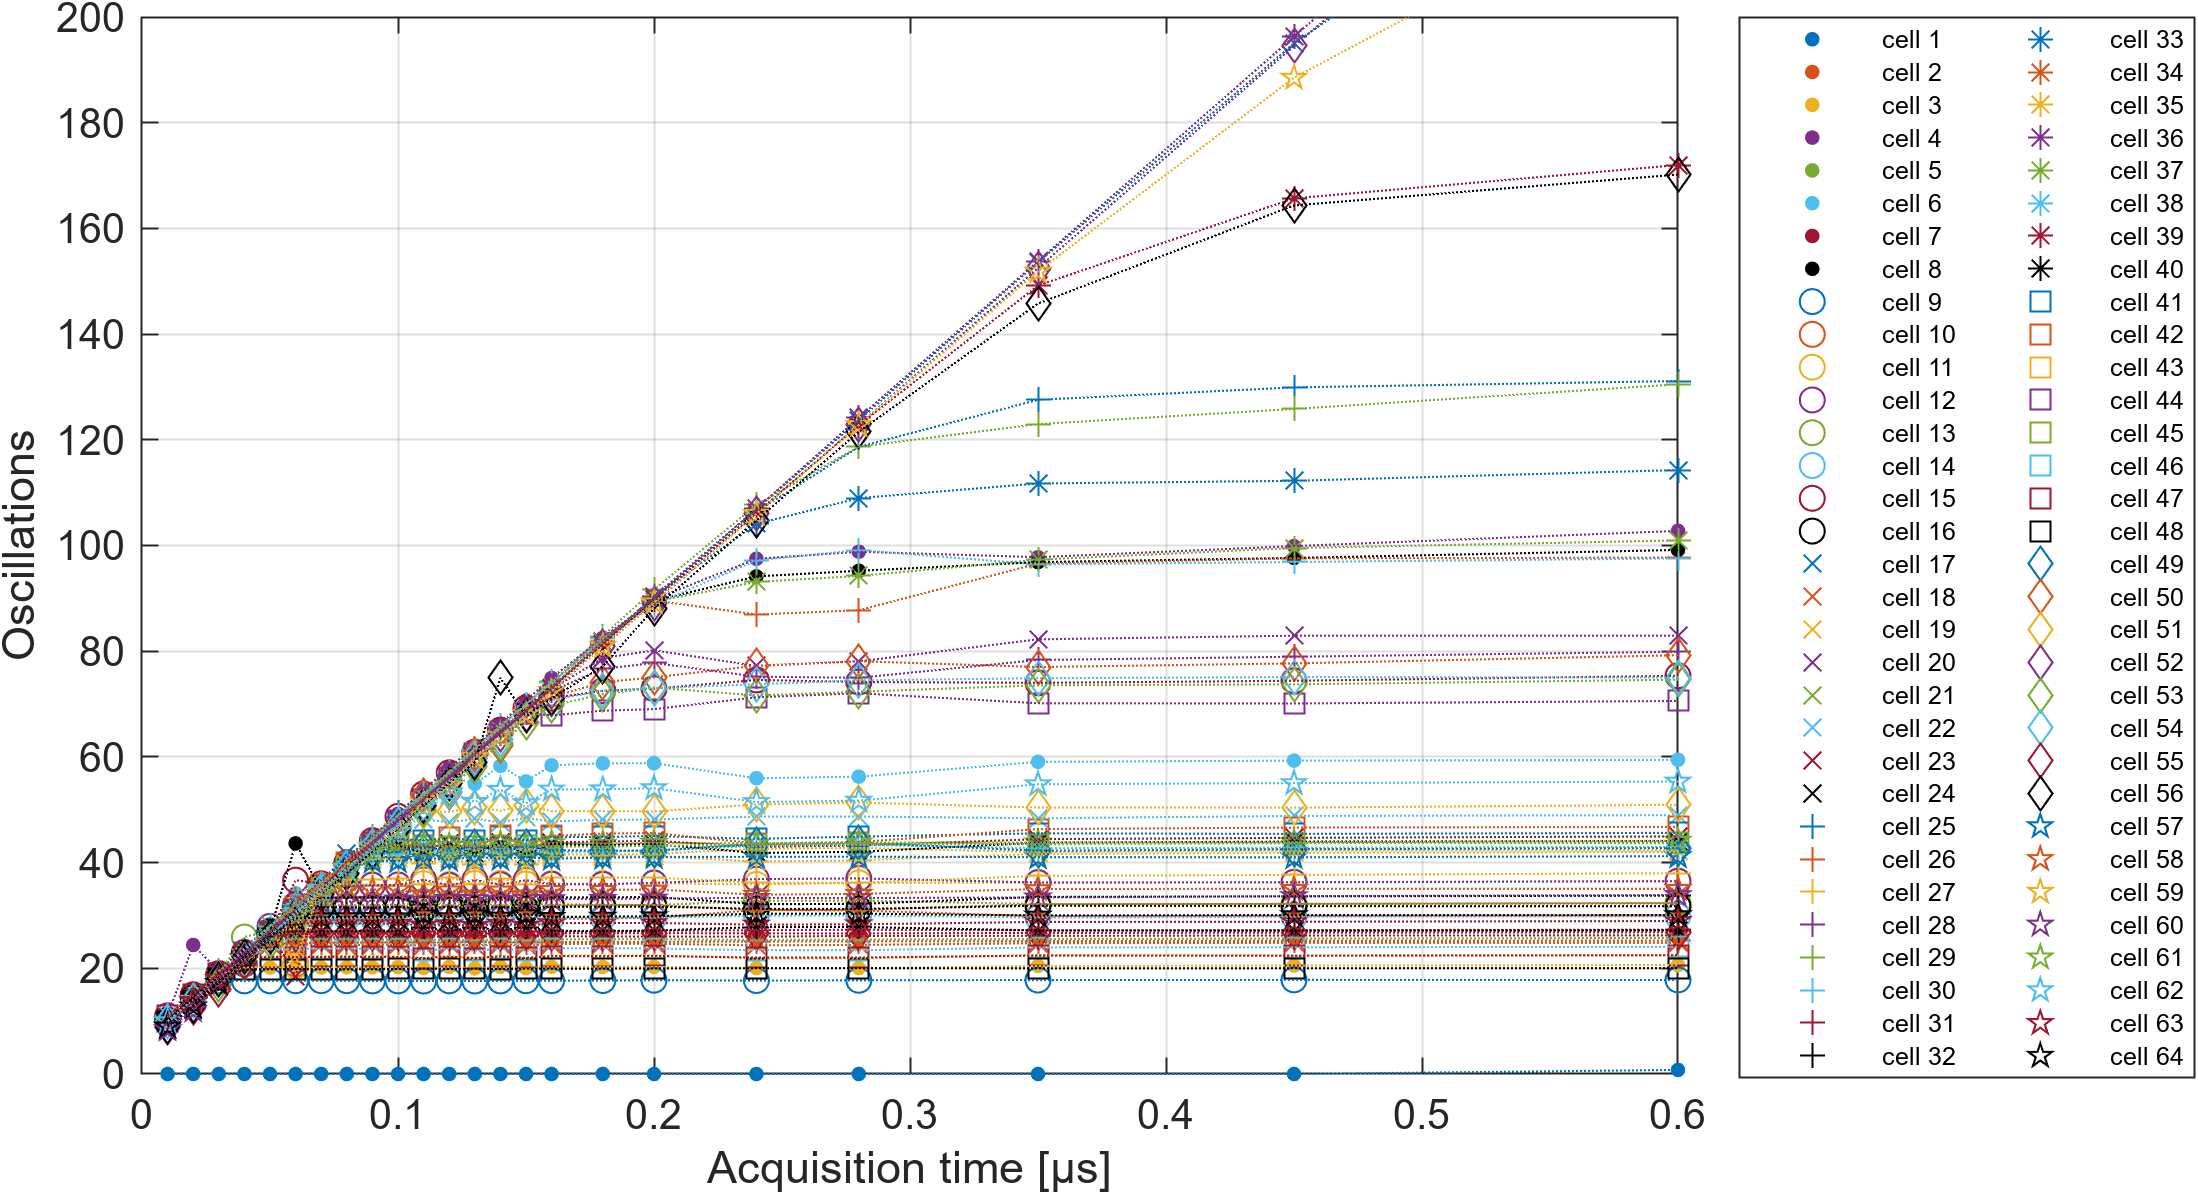
\includegraphics[width=\linewidth]{images/tero_8_oscillations_vs_time_zoomed.png}
        \subcaption{Zoomed\label{fig:tero_8_oscillation_vs_time_zoomed}}
   \end{minipage}
   \caption{TERO-8 cells oscillations over acquisition time\label{fig:tero_8_oscillation_vs_time}}
\end{figure}


Figures \ref{fig:tero_8_oscillation_vs_time_full} and \ref{fig:tero_8_oscillation_vs_time_zoomed} confirm that most of the cells do stabilise and only a few are unstable as expected. If the unstable cells become an issue for the implementation, we could imagine changing the physical location of the unstable cells on the \acrshort{fpga} until all cells are stable. However, this would require a calibration step and this will not be studied in this thesis.


\subsection{Final state}

The final state of the cells (i.e. the number of oscillations after stabilisation) is difficult to see on the previous graphs. Here we display the final state of each cell at $2\mu s$ as a histogram on figures~\ref{fig:tero_both_oscillation_final}. The cells that are considered unstable from the previous section are excluded for more visibility.\\

For the TERO-4, this reveals that 48 of the 64 cells have a final number of oscillations equal to zero, meaning that they do not oscillate a single time. For the TERO-8, the final number of oscillations is more spread than for the TERO-4, with at most 3 cells with the same number.

\begin{figure}[H]
   \begin{minipage}[b]{0.5\linewidth} 
        \centering
        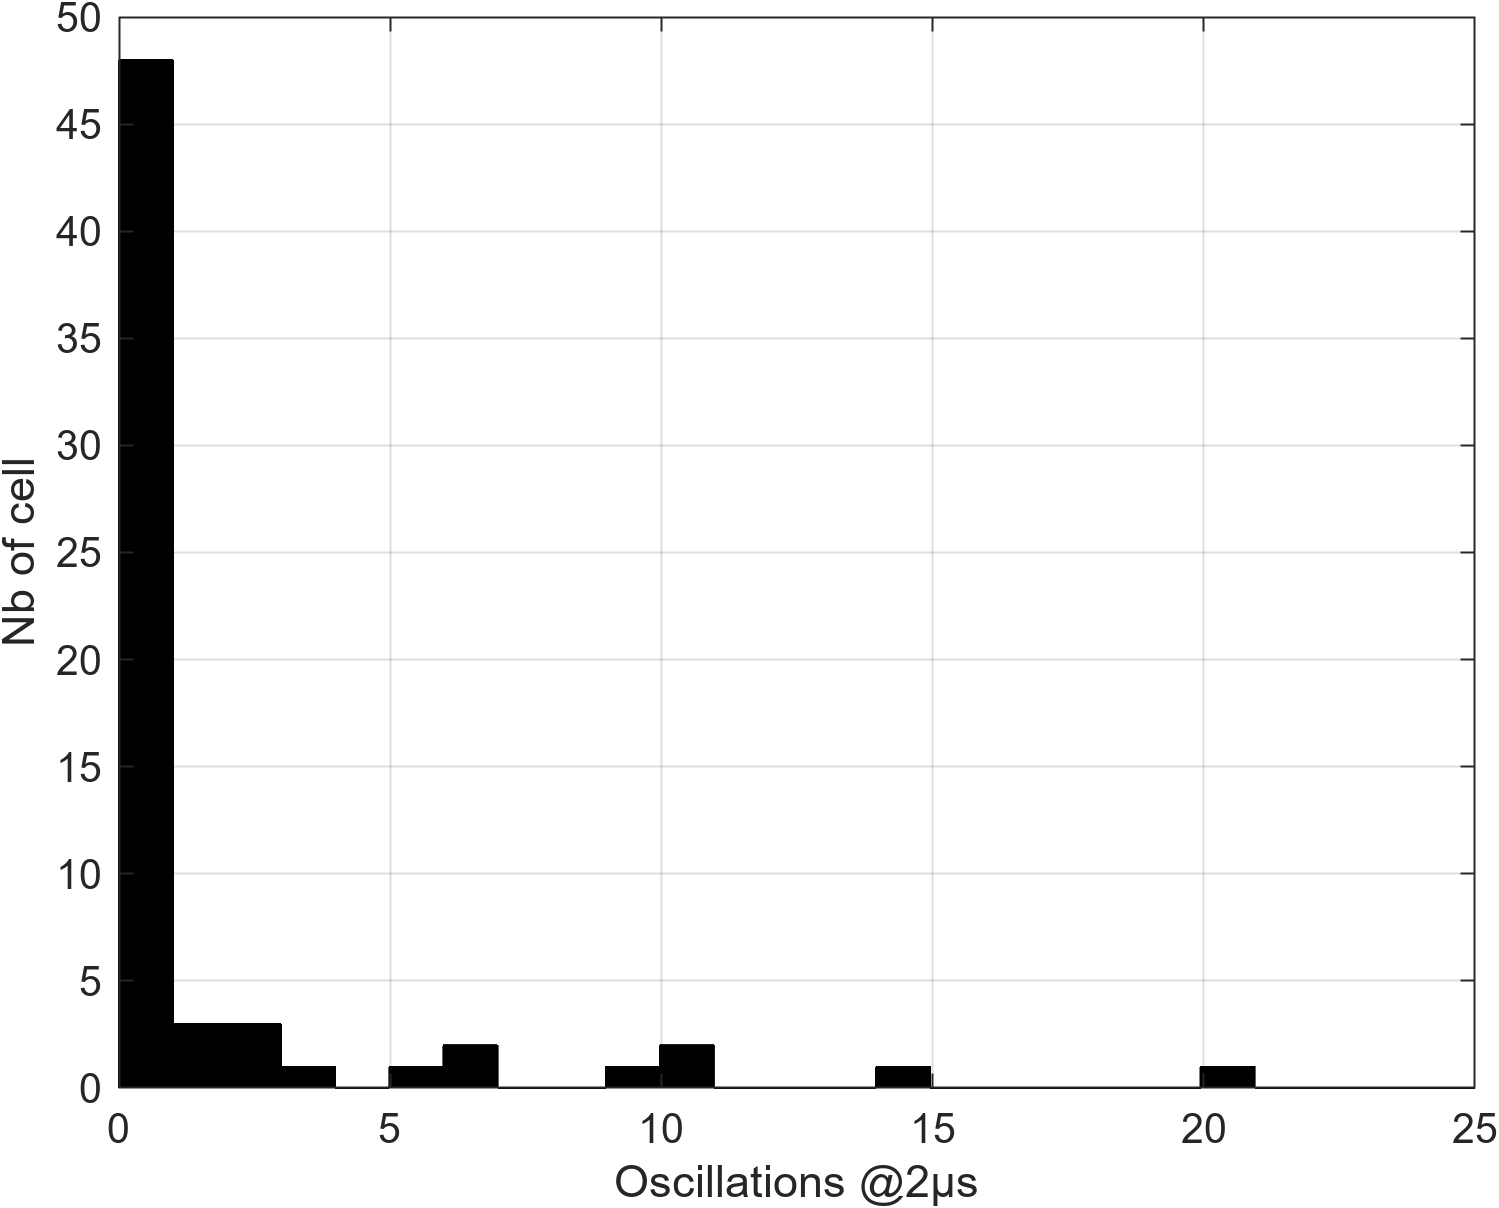
\includegraphics[width=\linewidth]{images/tero_4_oscillations_final.png}
        \subcaption{TERO-4\label{fig:tero_4_oscillation_final}}
   \end{minipage}
   \begin{minipage}[b]{0.5\linewidth}   
        \centering
        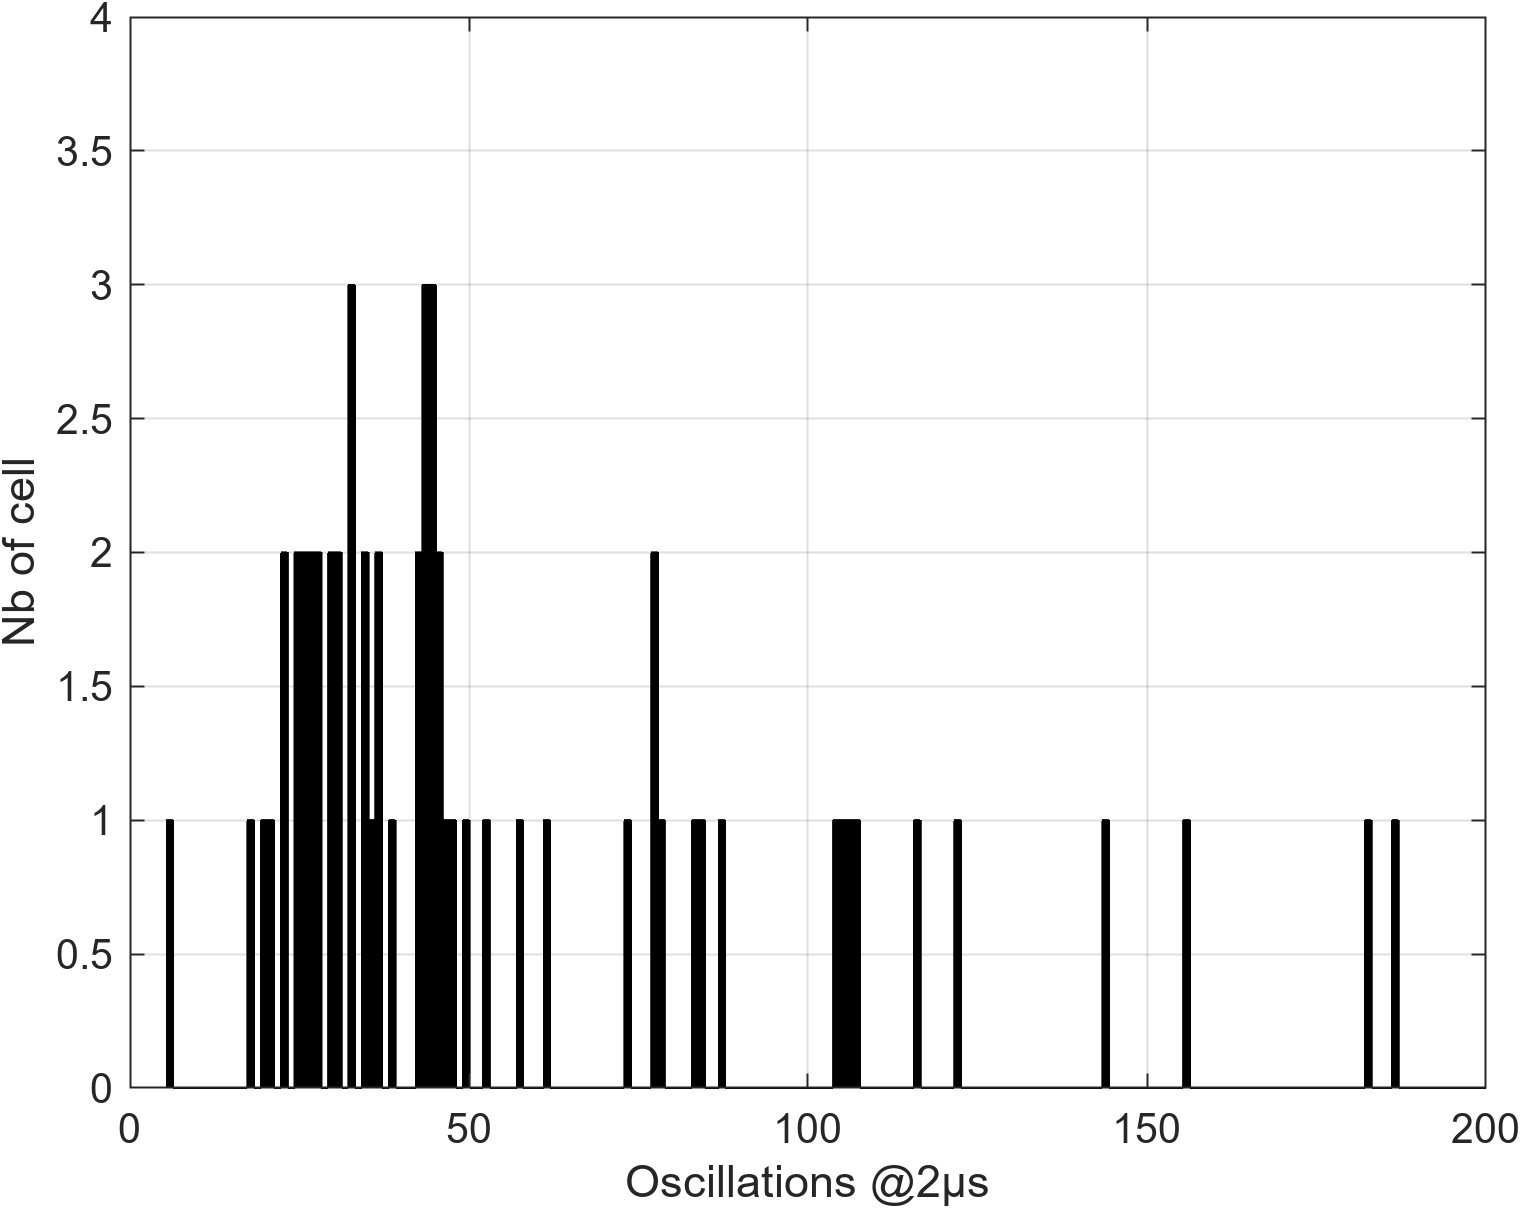
\includegraphics[width=\linewidth]{images/tero_8_oscillations_final.png}
        \subcaption{TERO-8\label{fig:tero_8_oscillation_final}}
   \end{minipage}
   \caption{\acrshort{tero} cells - number of oscillations at $2\mu s$\label{fig:tero_both_oscillation_final}}
\end{figure}




\newpage
\subsection{Equality's}

In the \acrshort{puf} implementation, the bits responses are generated by comparing the number of oscillations of two cells. Therefore, a high proportion of the cell having the same number of oscillations will lead to a high number of equalities in the process. As discussed in the section~\ref{sec:design_generation}, the equality results in a response that is always the same and therefore needs to be avoided as much as possible.


\begin{figure}[H]
    \centering
    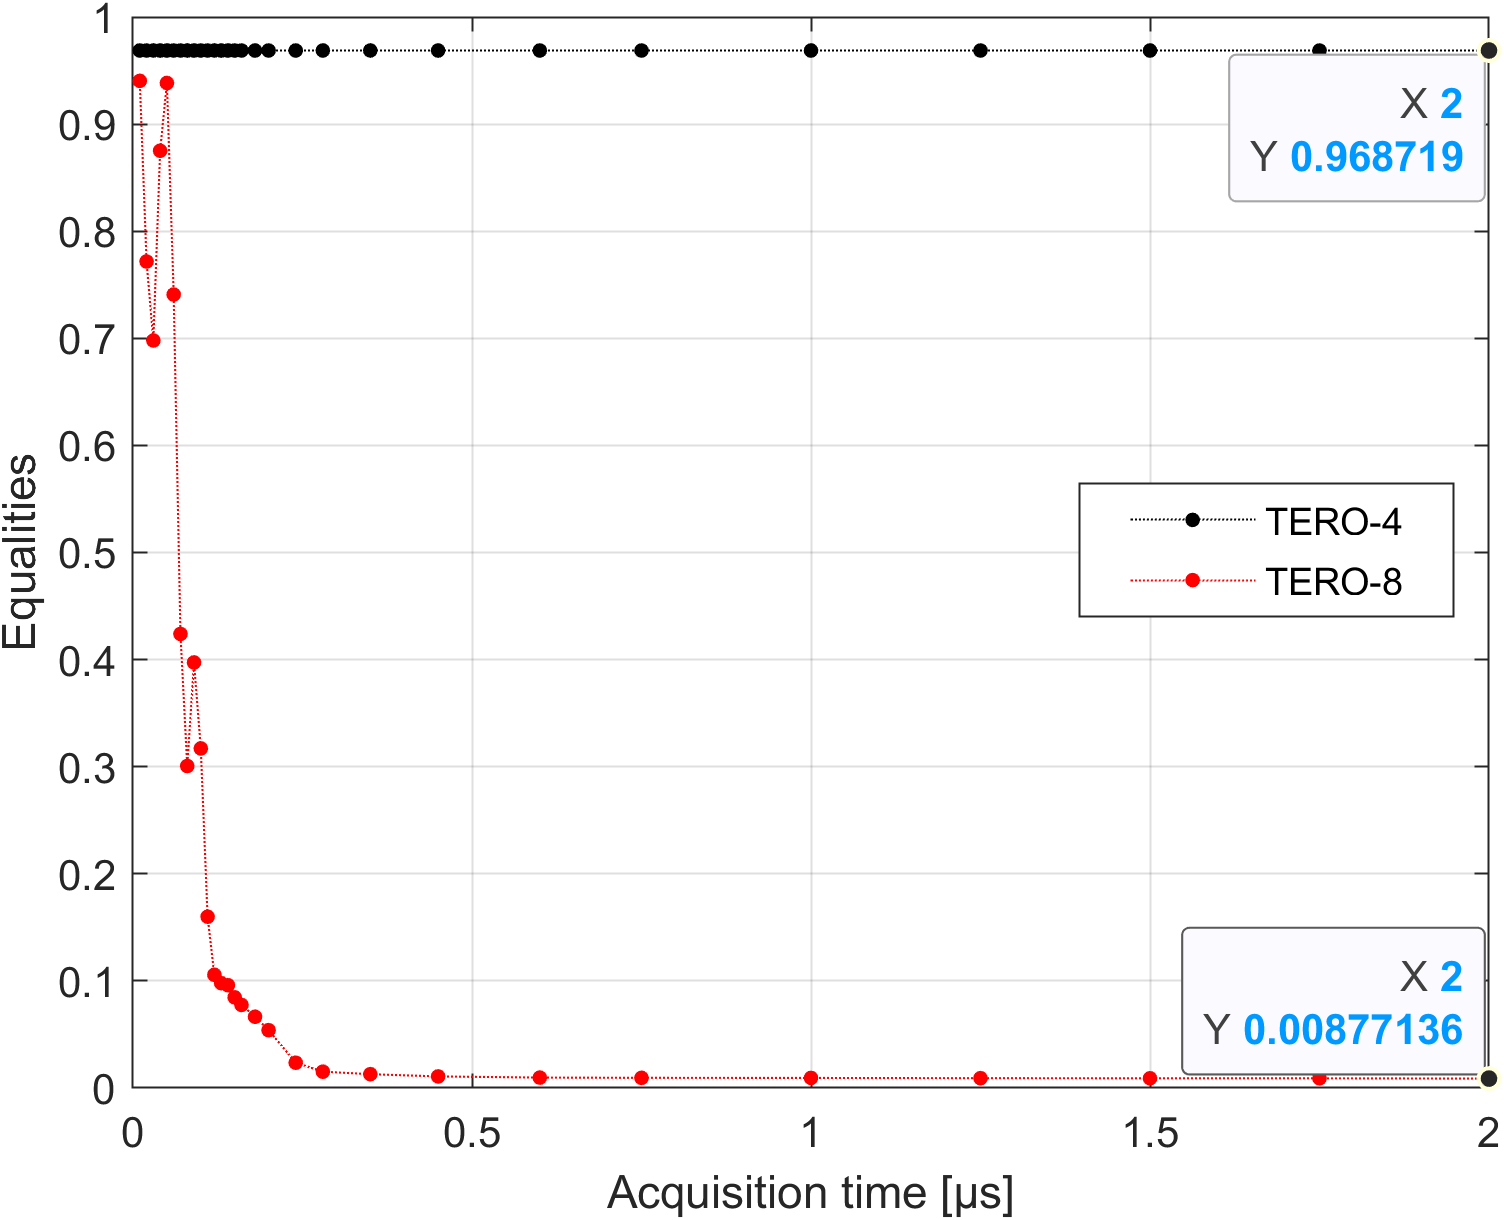
\includegraphics[width=0.8\linewidth]{images/all_oscillations_equality.png}
    \caption{\label{fig:tero_all_oscillation_eq}\acrshort{tero} cells oscillations equality's over acquisition time}
\end{figure}

Comparing each pair of cells similarly than for the response generation, we can find the proportion of equalities, which is shown in figure~\ref{fig:tero_all_oscillation_eq}. The TERO-4 cells comparison raises an equality for 96.8\% of the cells combination, for any acquisition time. The TERO-8 cells however produced less than 1\% of equality after $0.4 \mu s$ and almost 0\% at $2\mu s$. It is also interesting to observe the beginning where there is a high number of equality which decreases rapidly. This is coherent since this is the moment where the cells start to stabilise, each one at a time, and therefore the number of oscillations diverges for each cell.\\

From this test, TERO-4 cells seem to not be suitable due to a high proportion of the cells that do not oscillate, while the TERO-8 cells behave as expected. However, it is possible that another device would produce a completely different behaviour and it could simply be due to unfortunate circumstances.\\


\section{Intra-device performances and acquisition time determination}

This tests studies the intra-device metrics (\acrlong{unif} and \acrlong{relia})  of the \acrshort{puf} for different acquisition times (still between $0.01\mu s$ to $2\mu s$). This provides a first look at the \acrshort{puf} performances on a single device, before the final characterisation with the inter-device metrics. The goal is also to choose an adequate acquisition time to have the best \acrshort{puf} properties for the final test.\\

\subsection{Uniformity}

As defined in the chapter~\ref{ch:1-puf}, \acrfull{unif} is the measure of the response's bit repartition between '0' and '1' and is ideally equal to 50\%. This metric is displayed in figure~\ref{fig:all_intra_uniformity} for both TERO-4 and TERO-8. The uniformity of the TERO-4 PUF stays steady at 3\% while the TERO-8 oscillates shortly then rises and stabilises to 53.0\% around $0.3\mu s$.\\


\begin{figure}[H]
    \centering
    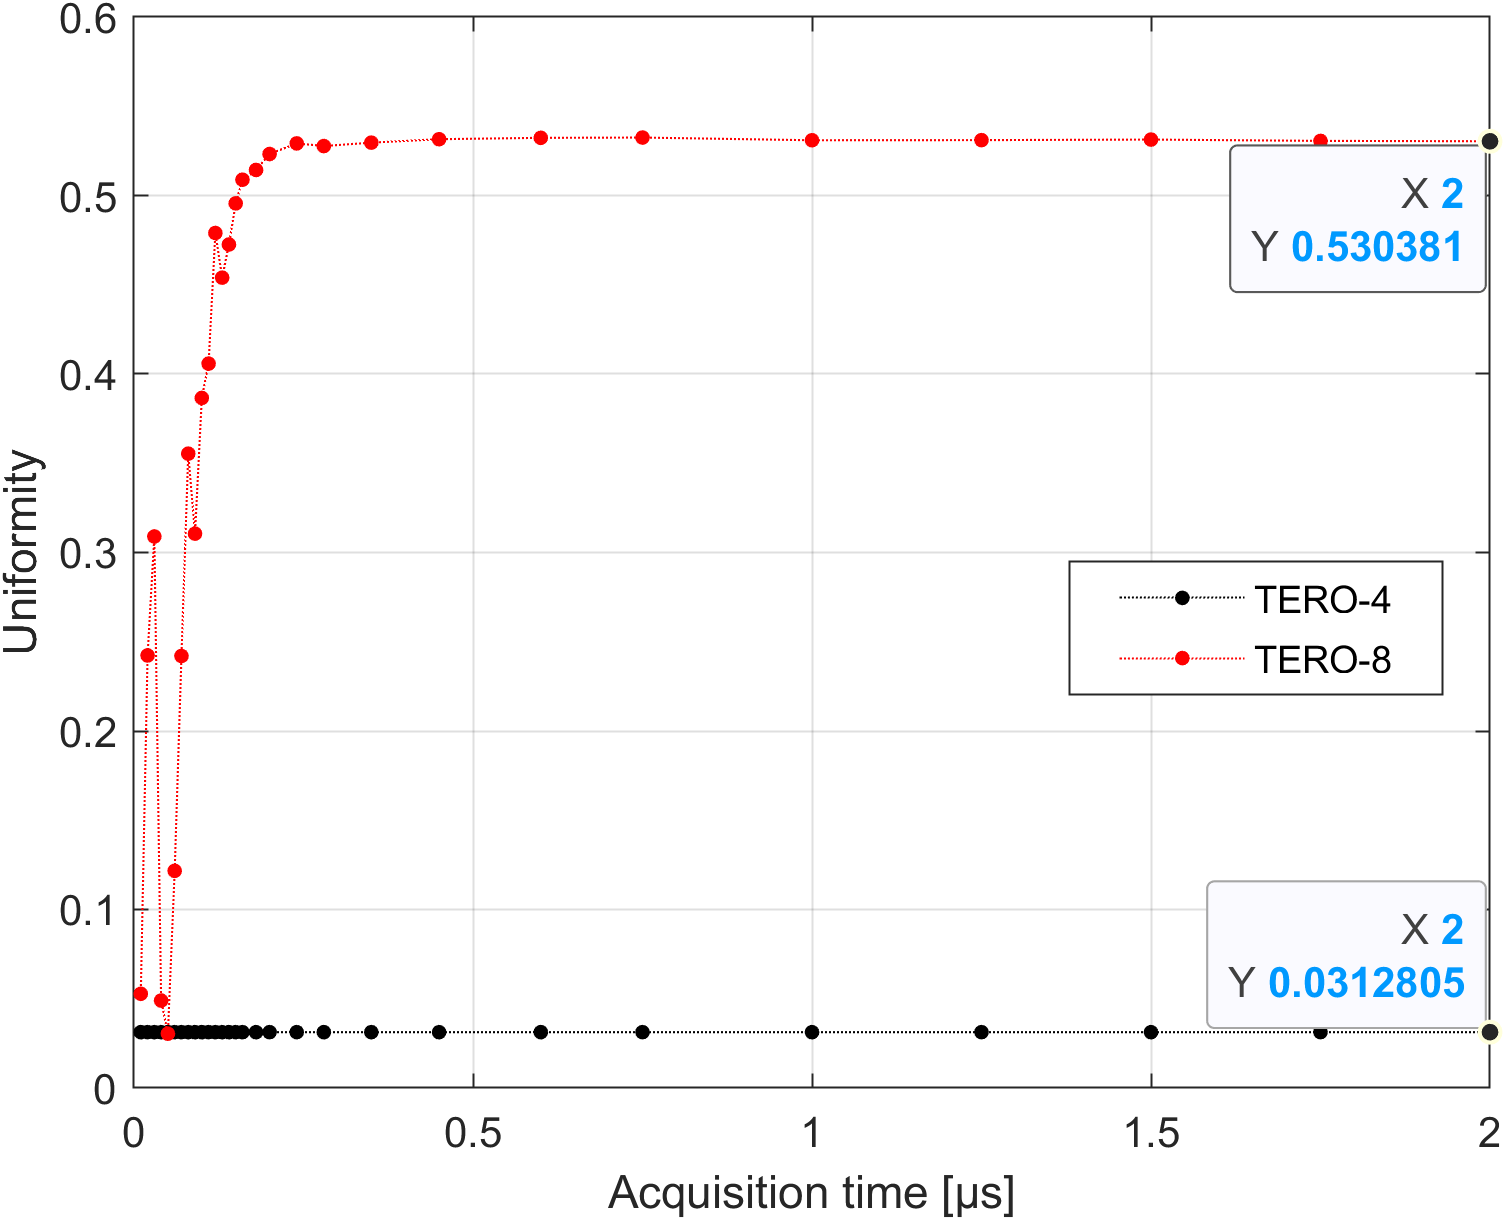
\includegraphics[width=0.8\linewidth]{images/all_intra_uniformity.png}
    \caption{\acrshort{puf} intra-uniformity}
    \label{fig:all_intra_uniformity}
\end{figure}

It was expected from the previous test about cell oscillations that the uniformity of the TERO-4 would be poor, due to the high number of equalities. From the 96.8\% of equality found, we know that 96.8\% of the generated bits are '0'. If we assume that the remaining 3.2\% of the bit are perfectly uniform, this would induce that $96.8\% + 3.2\%\times50\% = 98.4\%$ of the bits are '0', which corresponds to a uniformity of 1.6\%. The 3\% found is higher than this prediction, indicating that there is more '1' on the remaining bits than expected. Nevertheless, this proves that the TERO-4 uniformity is extremely low, at least for this specific device.\\


For the TERO-8, the oscillation of the uniformity at the beginning of the figure~\ref{fig:all_intra_uniformity} is also expected from the oscillation of the equalities at the same acquisition time. Once it is stabilised, the uniformity exceeds 50\% by 3\%, indicating that there is slightly more '1' than '0' in the bits response.\\

In both case, there is more '1' than expected, which could be either due to this specific device or to the implementation. This will be determined by the inter-device characterisation (~\ref{sec:inter_device_perf}).

\subsection{Reliability}


The \acrfull{relia} is the measure of the stability of each bit over multiple samples and is ideally equal to 100\%. This metric is shown in figure~\ref{fig:all_intra_reliability}. The TERO-4 reliability is constantly at 100\% while the TERO-8 reliability oscillates initially between 99 and 93\%, then stabilises at 97.7\% after $0.4\mu s$.

\begin{figure}[H]
    \centering
    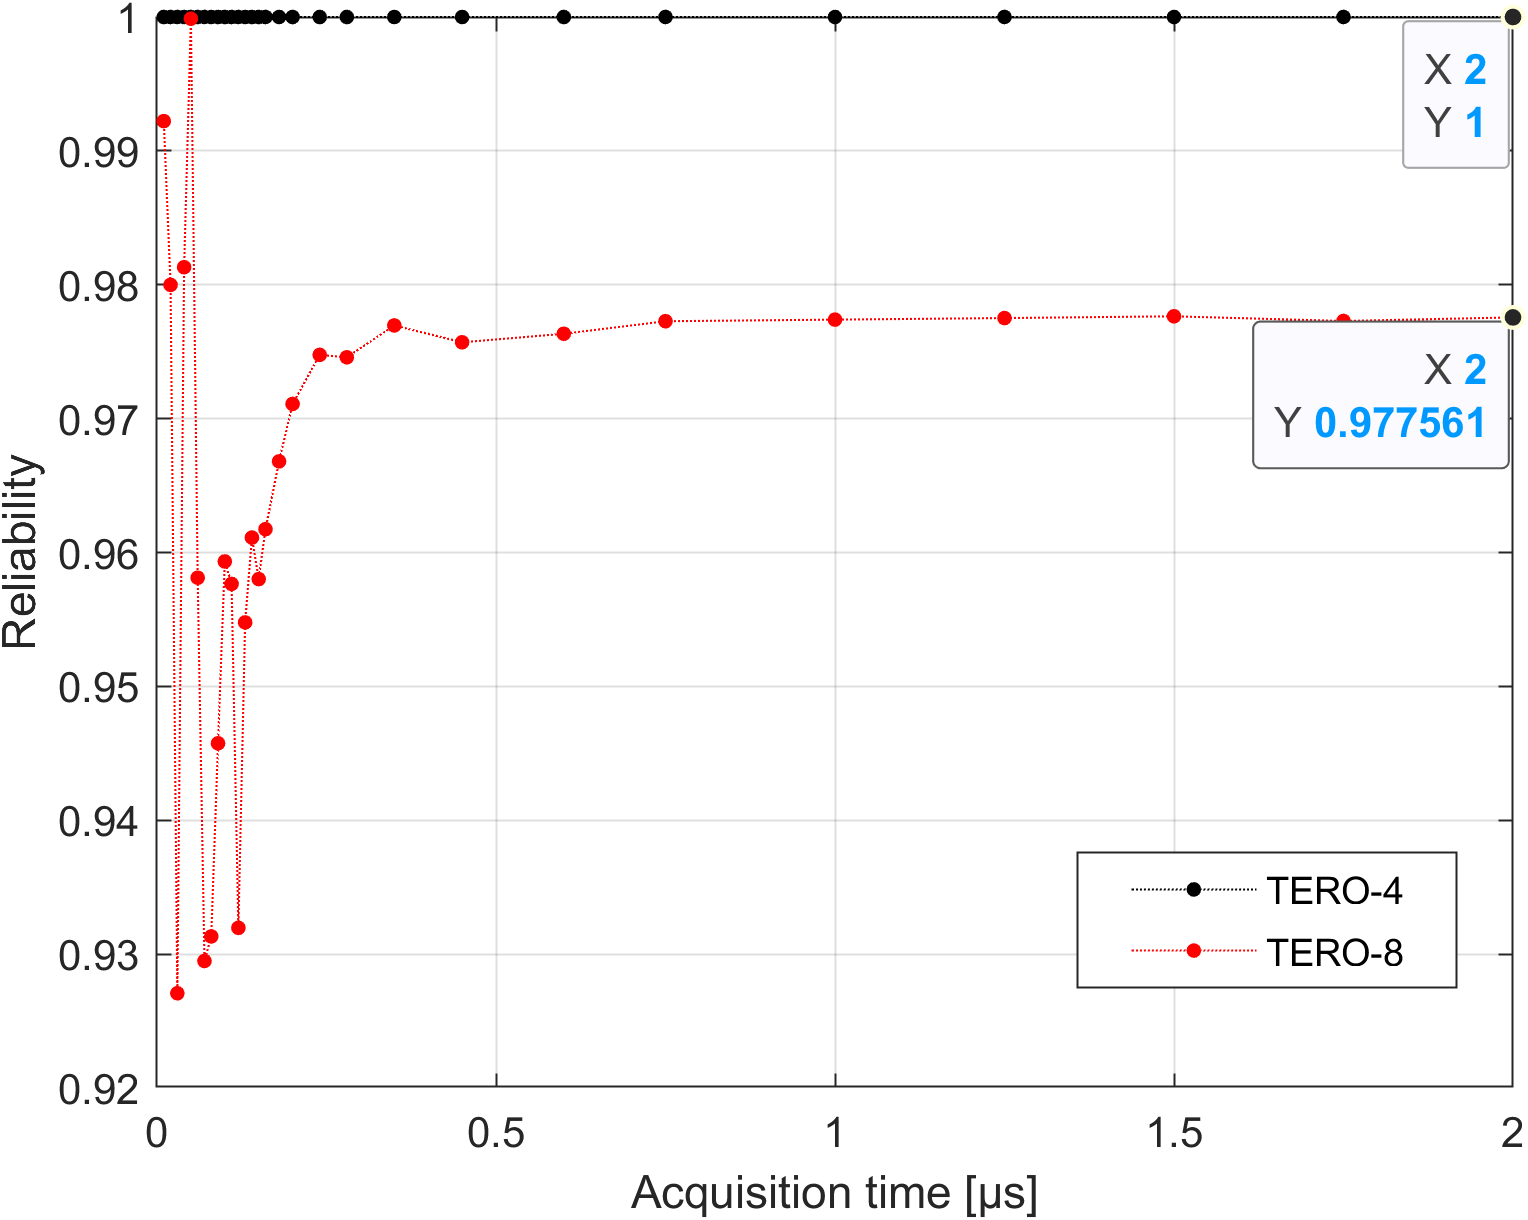
\includegraphics[width=0.8\linewidth]{images/all_intra_reliability.png}
    \caption{PUF intra-reliability}
    \label{fig:all_intra_reliability}
\end{figure}

The TERO-4 constant reliability is coherent with the fact that 63 of the 64 stabilise immediately, and therefore the response does not change anymore with the acquisition time. The fact that it is at 100\% reveals that the cell's final states are completely stable for this device over the 10 000 samples captured.\\

Once the TERO-8 cells have stabilised, the reliability found is comparable to the state of the art, but additional error correction techniques could increase the stability depending on the target application.\\

When we look at both the uniformity and reliability of the implementations, we can confirm that the TERO-4 does not provide good enough performance on this specific device while TERO-8 seems to produce correct performance. This also shows that an acquisition time higher than $0.5 \mu s$ does not provide any benefit to the results from this device. We choose $1 \mu s$ for the acquisition time used in the final tests, by assuming that the variation of this result between the devices is smaller than $0.5 \mu s$.


\section{Inter-device performances}

\label{sec:inter_device_perf}

The previous performance estimations are done on a single board and it is important to study the variation of those performances over multiple devices. The responses produced by different devices should be very unique and we can also check a systematic bias in the implementation for specific bits. In this test, the two TERO PUFs are uploaded on 33 BASYS-3 boards and the responses are recorded for an acquisition time of $1\mu s$. The device used in the previous test is at index 1.

\subsection{Inter-device uniformity}


\begin{figure}[H]
    \centering 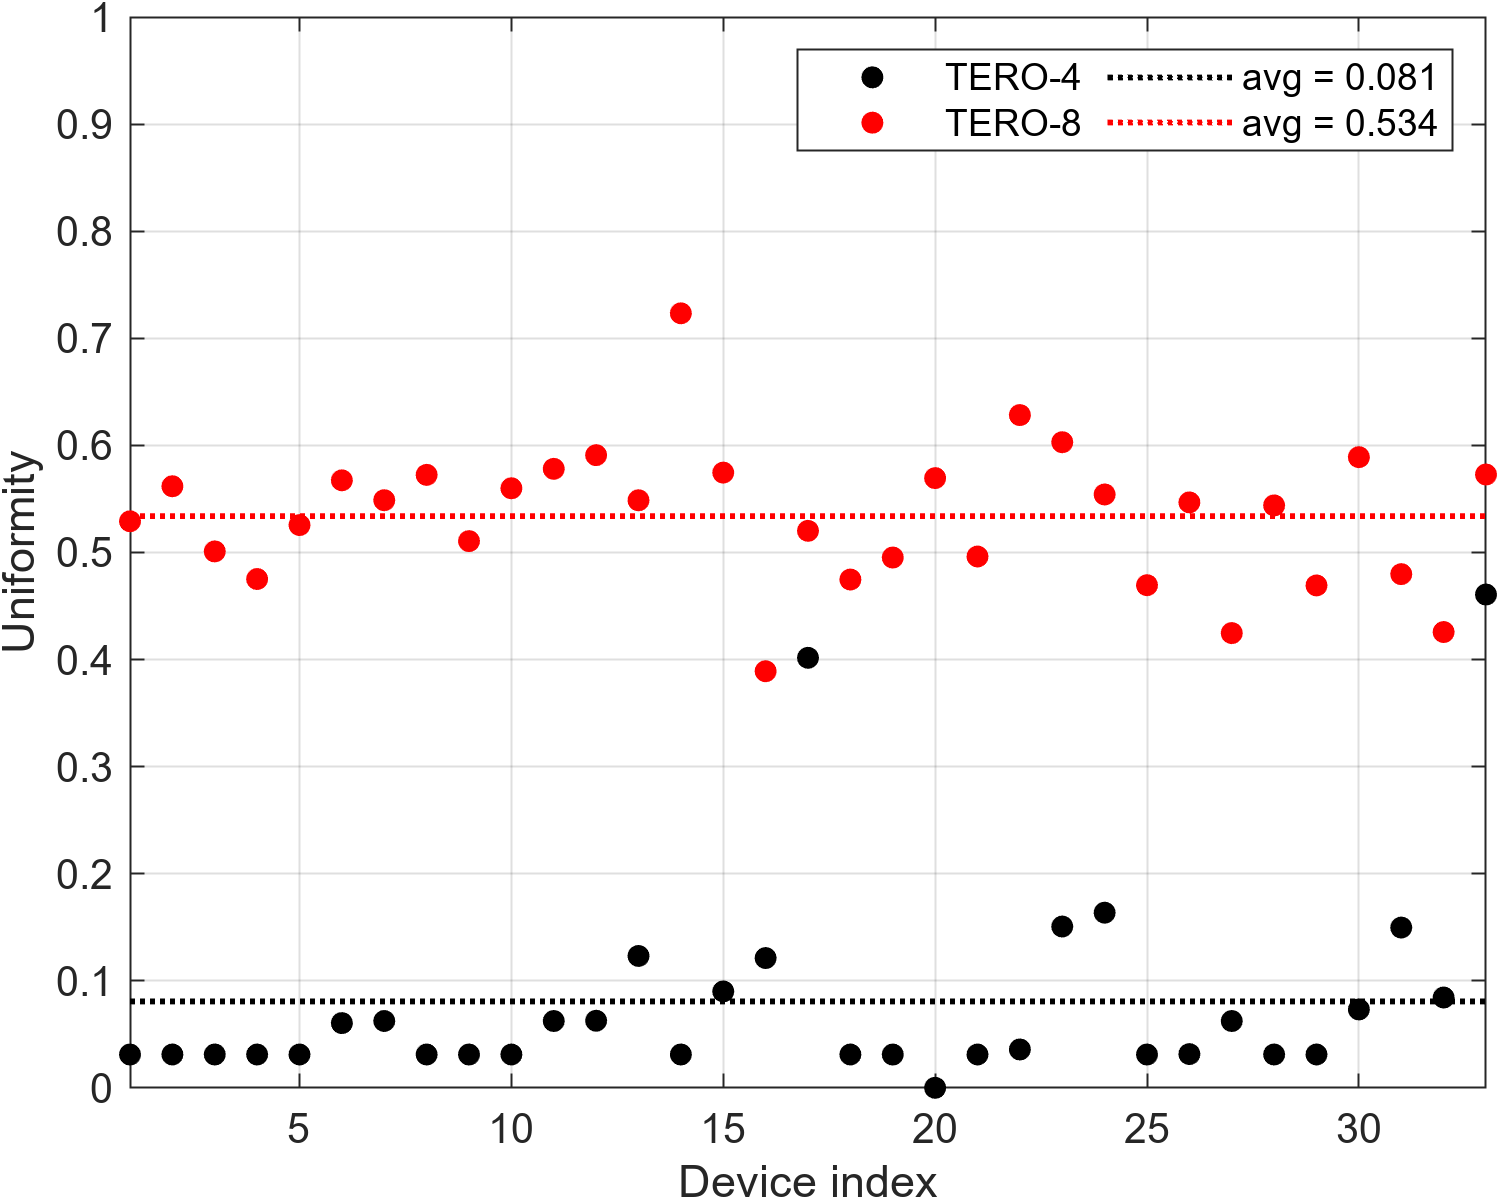
\includegraphics[width=0.8\linewidth]{images/tero_inter_uniformities.png}
    \caption{Inter-device uniformity's}
    \label{fig:tero_inter_uniformities}
\end{figure}


The TERO-4 uniformities of the 33 boards are represented in the figure~\ref{fig:tero_inter_uniformities}, with the dotted line for the average. 2 devices produce a uniformity higher than 40\%, while most of them stay below 8.0\% average. This proves that the poor uniformity found in the previous test (device at index 1) is not due to bad luck in the choice of the device but rather comes from the TERO-4 cells implementation itself.\\


The TERO-8 uniformities in figure~\ref{fig:tero_inter_uniformities} reveal that the device's uniformity from the previous test (53.0\%) was really representative of the 53.4\% average uniformity for this implementation. However, this also shows that this metric variation of this metrics between 39\% and 72\% depending on the device used.



\subsection{Inter-device reliability}
\label{subsec:inter_device_relia}

\begin{figure}[H]
    \centering 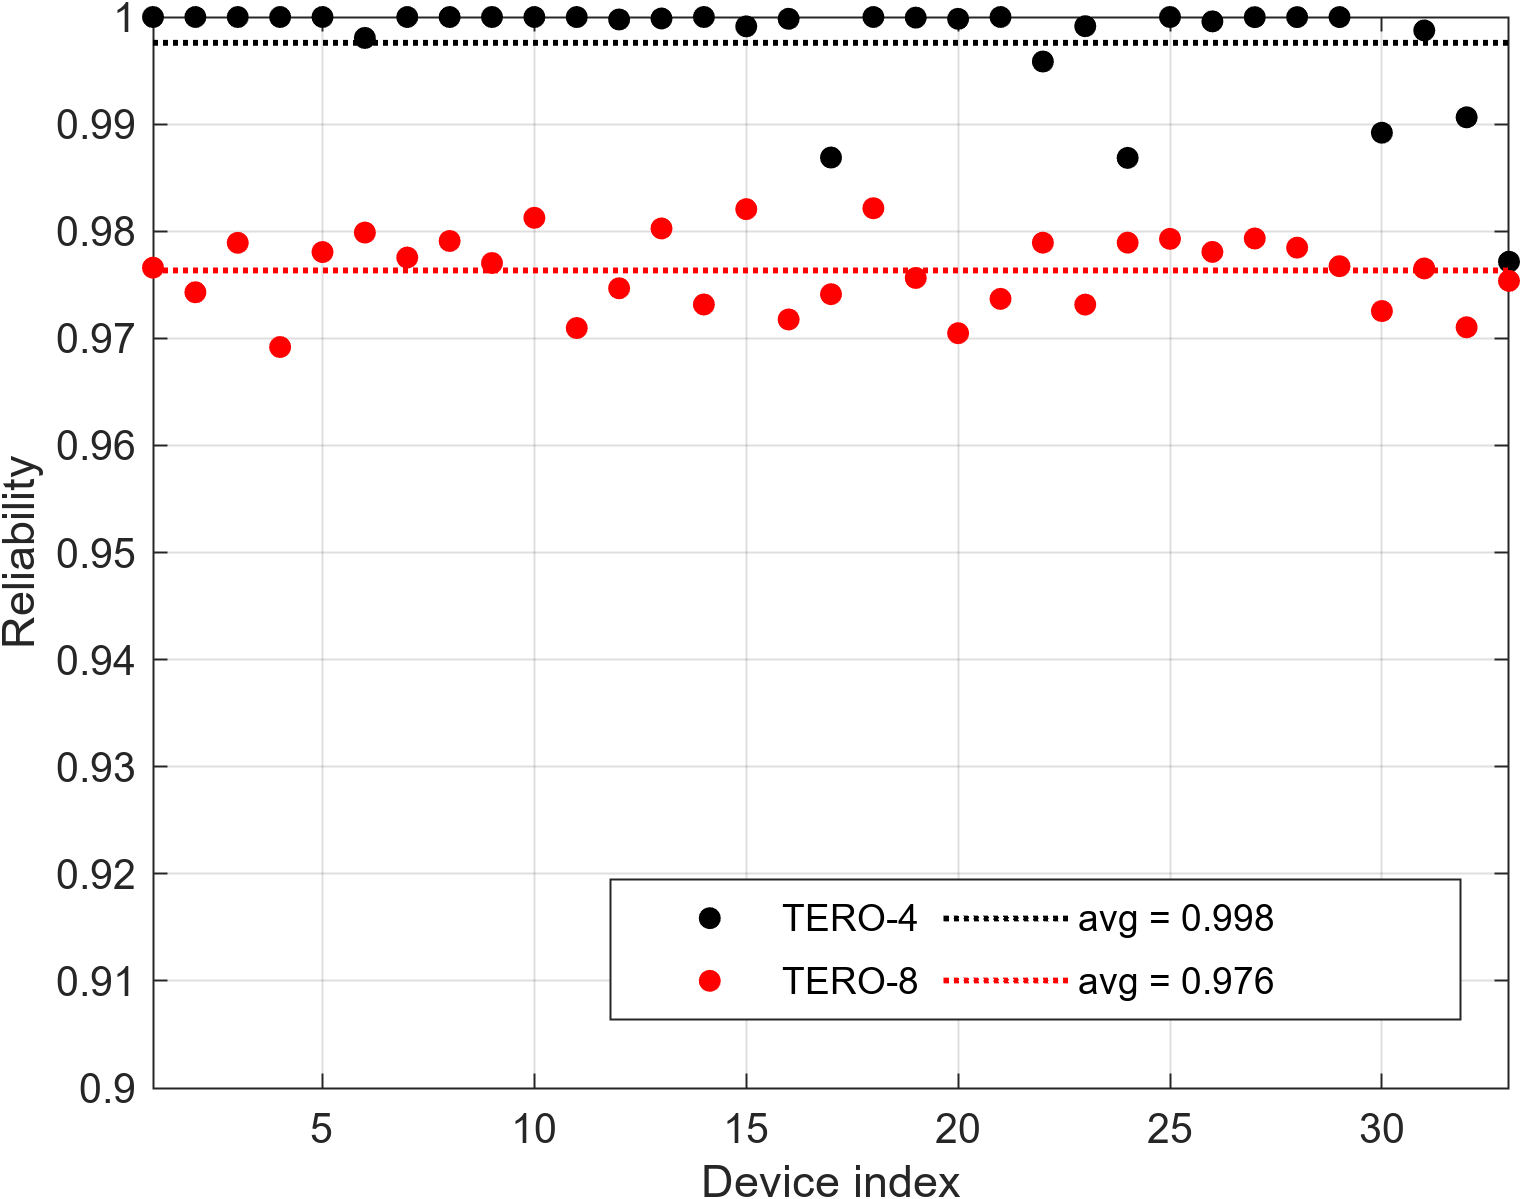
\includegraphics[width=0.8\linewidth]{images/tero_inter_reliabilities.png}
    \caption{Inter-device reliability's}
    \label{fig:tero_inter_reliabilities}
\end{figure}

Figure~\ref{fig:tero_inter_reliabilities} represent the TERO-4 reliability's. This indicates that most devices produce near-perfect reliability (99.8\% average). This also reveals that the device used in the previous test (index 1) was one of the devices that have perfect reliability over the 10 000 samples, but that is not always the case and a few devices produced a reliability below 99\%.\\


The TERO-8, displayed in figure~\ref{fig:tero_inter_reliabilities}, confirms that the value found on the previous test (97.7\%) was a good representation of the average (97.6\%) for the 33 devices. Furthermore, we can see that all the values are within a variation of 1\%.


\subsection{Bit-Aliasing}

Bit-aliasing is the measure of how likely is a specific bit to be '1' over all the devices. Ideally, this would be equal to 50\% for all the bits. However, since we only tested 33 devices, instead of looking only at the average, we should compare the distribution of the bit-aliasing values to the ideal distribution i.e. a binomial distribution of probability 50\% over 33 experiments (represented in green in figure~\ref{fig:tero_inter_aliasing}).

\begin{figure}[H]
    \centering 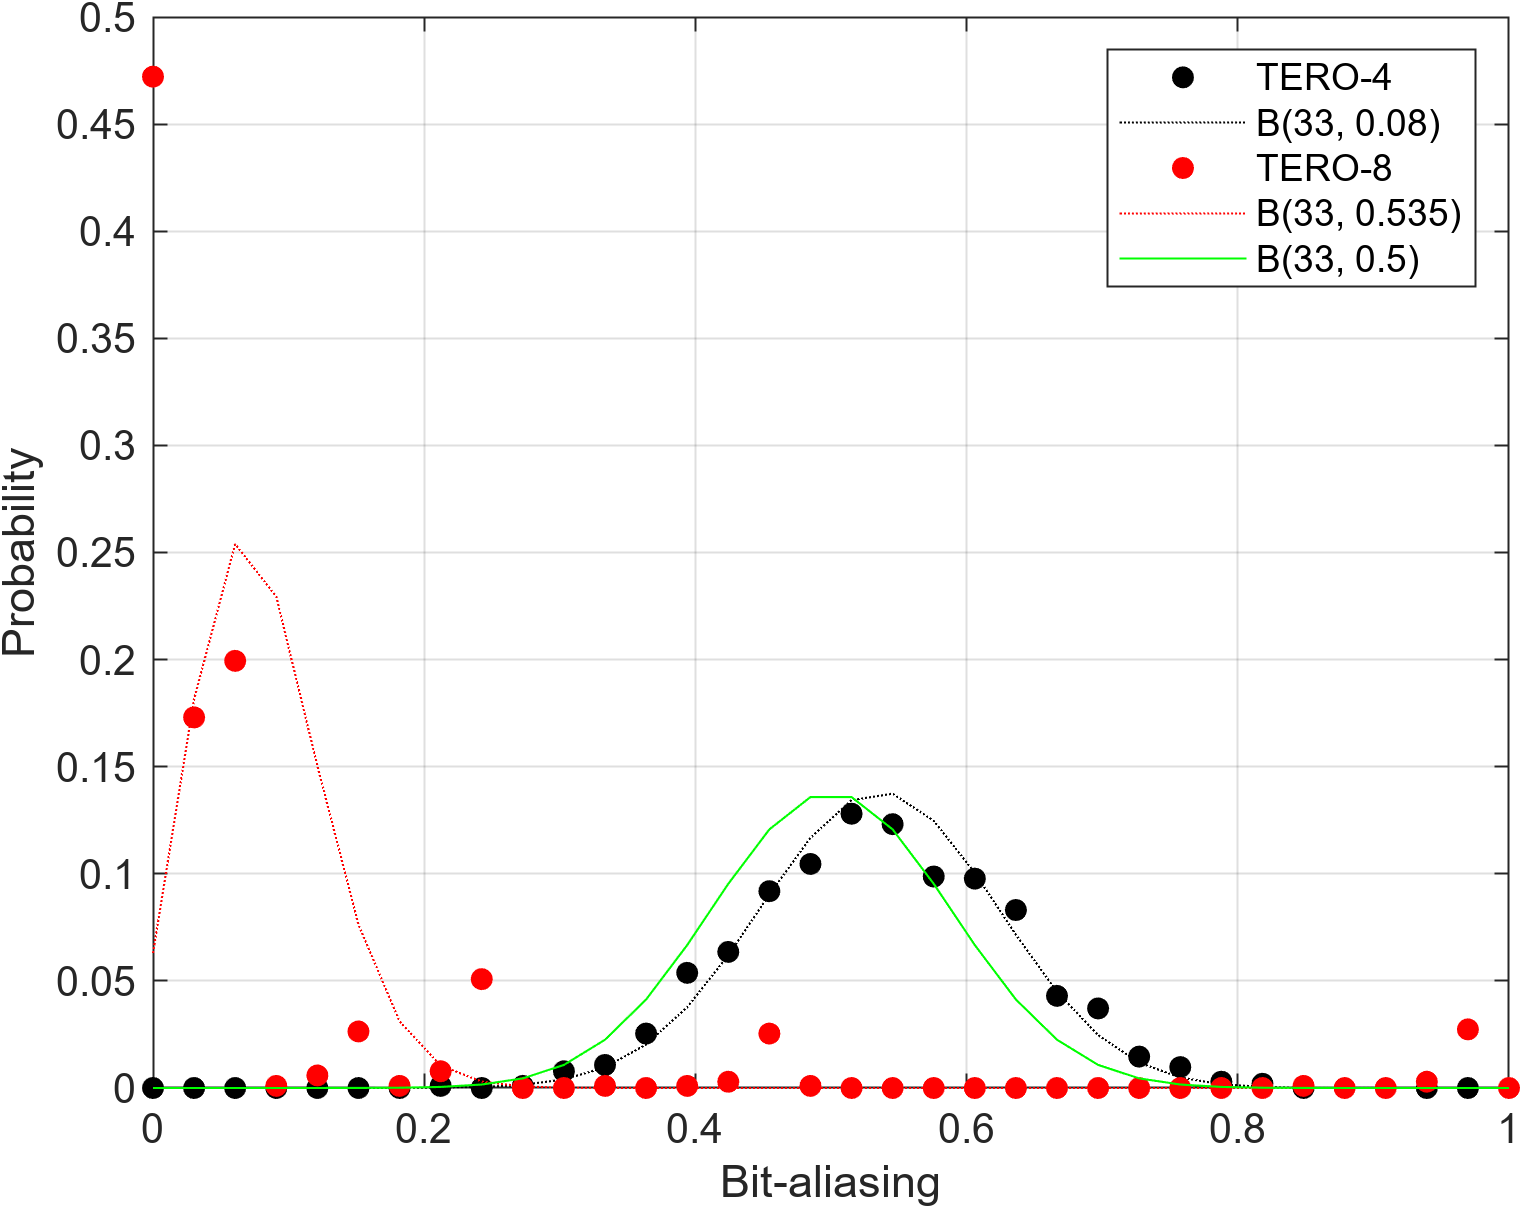
\includegraphics[width=0.8\linewidth]{images/tero_inter_aliasing.png}
    \caption{Inter-device bit-aliasing}
    \label{fig:tero_inter_aliasing}
\end{figure}

We already know that only 8.0\% of the TERO-4 bits are '1' for the average uniformity. Figure~\ref{fig:tero_inter_aliasing} reveals that almost 50\% of the bits are completely biased toward 0, meaning that they are always '0' in all the 33 devices tested. The average bit-aliasing is 8.0\% but the TERO-4 distribution does not follow a binomial distribution for this probability either. From the previous test, we know that the large number of bits equal to '0' in the device at index 1 is due to the large number of cells that do not oscillate. If we suppose that this is also the case in the other device, then this would mean that at least part of the cell that does not oscillate seems to always be the same regardless of the device. This indicates a bias in the implementation itself for specific cells.\\



The TERO-8 bit-aliasing distribution (figure~\ref{fig:tero_inter_aliasing}) follows closely a binomial distribution centred around its average of 53.5\%. This indicates that all the bits seem to give different response depending on the device, with a small overall bias of 3.5\% toward '1' which correspond almost to the 3.4\% excess of uniformity. This means that no bit is systematically at the same value but that there seems to be a global tendency for the cells in one array to produce a higher number of oscillations than the cells in the other array.



\subsection{Uniqueness}

The uniqueness is the measure of how different the responses of the different devices are in terms of hamming distance, with an ideal value of 50\%. The results for this metric are on the table~\ref{tab:uniqueness}.

%Q?
%Decimal ? or %
\begin{table}[H]
    \centering
    \begin{tabular}{|c|c|}
        \hline
            & Uniqueness\\
         \hline
         TERO-4 & 8.2\%\\
         \hline
         TERO-8 & 49.4\%\\
         \hline
    \end{tabular}
    \caption{Uniqueness}
    \label{tab:uniqueness}
\end{table}

The TERO-4 responses only produce an 8.2\% of uniqueness, which is understandable since we know from the bit-aliasing that a large part of the bits response is always '0'. For the TERO-8 however, the responses have a uniqueness of 49.42\% over the 33 devices tested, which is close to the ideal value. 


\begin{table}[H]
    \centering
    \begin{tabular}{|c|c|c|c|c|}
        \hline
            & Uniformity & Reliability & Bit-aliasing & Uniqueness\\
         \hline
         TERO-4 & 8.1\% & 99.8\% & 8.0\% & 8.2\%\\
         \hline
         TERO-8 & 53.4\% & 97.6\% & 53.5\% & 49.4\%\\
         \hline
    \end{tabular}
    \caption{Inter-device performances}
    \label{tab:summary_inter}
\end{table}

It appears clearly that the TERO-4 implementation does not provide the desired performances in terms of uniformity, bit-aliasing and uniqueness. This is most likely due to the cells that systematically stabilise without any oscillation. We therefore consider this implementation to not be usable and it will not be discussed in the rest of this chapter.

\newpage
\section{Error correction}


The TERO-8 average reliability is 97.63\%, which, depending on the target application, may not be good enough. We will therefore evaluate the improvement brought by the ECC described in \ref{subsec:demon_feature_bch}.\\

The responses of the ECC implementation are recorded for the same acquisition time ($1\mu s$) over the 33 BASYS-3 boards in the same condition as the previous test. The table ~\ref{tab:raw_&_ecc_perf} contains all the inter-device metrics of the initial TERO-8 implementation ("Full"), the reduced version of it with only 171 bits ("Reduced") and the response of the BCH decoder for error correction ("ECC").

\begin{table}[H]  
  \centering
    \begin{tabular}{|c|c|c|c|c|c|}
        \hline
        \textbf{TERO-8} &  Response's size & RE & UF & UQ & BA\\
        \hline
        Full & 1023 bits & 97.6\% & 53.4\% & 49.4\% & 53.5\%\\
        \hline
        Reduced & 171 bits & 97.7\% & 53.4\% & 49.9\% & 54.4\%\\
        \hline
        ECC & 171 bits & 99.9\% & 53.5\% & 49.9\% & 54.4\%\\
        \hline
    \end{tabular}
   \caption{\label{tab:raw_&_ecc_perf}TERO-8 performances without and with ECC}
\end{table}

First, we can observe that the performances of the reduced version (without ECC) are very similar to the full one. Therefore, any improvement due to the ECC on the reduced response can be supposed to be equally effective on an entire response.

Moreover, when we compare the reliability between the reduced response and the ECC one, it goes from 97.71\% to 99.90\%, which is an improvement. At the same time, the other performances remain substantially the same.

As expected, using this technique, we significantly increase the performance of the TERO-8 without any downside other than the additional FPGA resources used (discussed in \ref{subsec:fpga_usage_area}). Depending on the target application, reliability higher than 99.9\% can still be required. In this case, a BCH supporting a higher number of errors should be used.\\

\newpage
\section{Comparison with existing implementations}

The performance produced by the TERO-8 implementation are comparable to both other \acrshort{teropuf} implementation (table~\ref{tab:tero_impls}) and other \acrshort{puf} techniques using an Artix-7 for implementation (table~\ref{tab:artix7_impl}), with only the \acrshort{ecc} version giving a reliability in line with the literature. 

\begin{table}[H]
    \centering
    \begin{tabular}{|c|c|c|c|c|c|c|c|}
         \hline
         \textbf{method} & \textbf{\acrshort{relia}} & \textbf{\acrshort{unif}} & \textbf{\acrshort{uniq}} & \textbf{\acrshort{bit-alia}} & \textbf{device} & \textbf{Ref}\\
         \hline\hline
         TERO & 98.3\% & - & 48\% & - & Cyclone-II & \cite{bossuet_puf_2014}\\
         \hline\hline
         TERO & 99.99\% & - & 46.7\% & - & Altera DE2 & \cite{bossuet_puf_2014}\\
         \hline
         TERO & 97.4\% & - & 48.5\% & - & Spartan-6 & \cite{marchand_implementation_2017}\\
          & 98.2\% & - & 47.6\% & - & Cyclone-V & \\
         \hline
         PDL-TERO & 98.8\% & - & 49.32\% & - & Spartan-3 & \cite{ardakani_improving_2018}\\
         \hline\hline
         \textbf{RAW (full)} & \textbf{97.6\%} & \textbf{53.4\%} & \textbf{49.4\%} & \textbf{53.5\%} & \textbf{Artix-7} & \textbf{This}\\ 
         \textbf{ECC} & \textbf{99.9\%} & \textbf{53.5\%} & \textbf{49.9\%} & \textbf{54.4\%} & & \textbf{work}\\
         \hline
    \end{tabular}
    \caption{\acrshort{teropuf} implementations on FPGA}
    \label{tab:tero_impls}
\end{table}



\begin{table}[H]
    \centering
    \begin{tabular}{|c|c|c|c|c|c|c|c|}
         \hline
         \textbf{method} & \textbf{\acrshort{relia}} & \textbf{\acrshort{unif}} & \textbf{\acrshort{uniq}} & \textbf{\acrshort{bit-alia}} & \textbf{Ref}\\
         \hline\hline
         APUF & 99.55\% & 51.84\% & 46.21\% & -  & \cite{anandakumar_implementation_2022}\\
         \hline
         XOR-APUF & 99.41\% & 50.73\% & 48.69\% &  - & \cite{anandakumar_implementation_2022}\\
         \hline
         BST-APUF & 99.99\% & - & 49.1\% & 50.3\% & \cite{he_highly_2020}\\
         \hline
         ROPUF & 99.19\% & 51.01 & 47.86\% & 51.01\% & \cite{de_weerdt_implementation_2021}\\
         \hline
         BST-ROPUF & 99.99\% & 46.78\% & 48.64\% & - & \cite{he_highly_2021}\\
         \hline
         RWC-SRAMPUF & 98.92\% & 55.38\% & 37.36\% & 46.89\% & \cite{cicek_new_2022}\\
         \hline
         Flip-Flop PUF & ~99\% & 49.2\% & - & 48.96\% & \cite{khan_symmetric_2020}\\
         \hline\hline
         \textbf{RAW (full)} & \textbf{97.6\%} & \textbf{53.4\%} & \textbf{49.4\%} & \textbf{53.5\%} & \textbf{This}\\ 
         \textbf{ECC} & \textbf{99.9\%} & \textbf{53.5\%} & \textbf{49.9\%} & \textbf{54.4\%} & \textbf{work}\\
         \hline
    \end{tabular}
    \caption{\acrshort{puf} implementations on Artix-7}
    \label{tab:artix7_impl}
\end{table}

\newpage
\section{Demonstration}

Using the python module (appendix~\ref{appendix:python_mod}) and a USB cable for \acrshort{uart} communication between the \acrshort{fpga} and a computer, we can demonstrate the different responses of the implementation: the raw response (figure~\ref{fig:demo_raw}), the response after \acrshort{ecc} (figure~\ref{fig:demo_ecc}) and the \acrshort{sha} key generated (figure~\ref{fig:demo_sha}).

\begin{figure}[H]
    \centering
    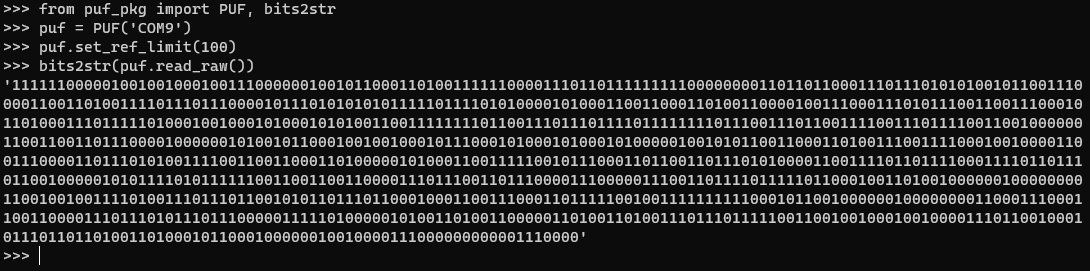
\includegraphics[width=\linewidth]{images/demo_raw.png}
    \caption{Demonstration raw response}
    \label{fig:demo_raw}
\end{figure}

\begin{figure}[H]
    \centering
    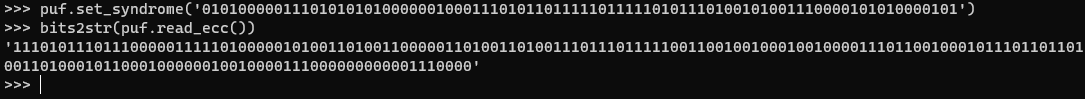
\includegraphics[width=\linewidth]{images/demo_ecc.png}
    \caption{Demonstration ECC response}
    \label{fig:demo_ecc}
\end{figure}

\begin{figure}[H]
    \centering
    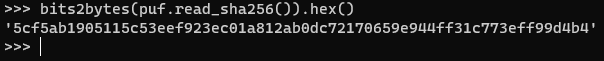
\includegraphics[width=\linewidth]{images/demo_sha.png}
    \caption{Demonstration SHA-256 key}
    \label{fig:demo_sha}
\end{figure}





\chapter{Conclusion}

%ARCHITECTURE



%SUMMARY OF WORK (problem + concept)

\acrshort{teropuf} is a promising technique that needs further research to cover more devices and possible variations. In particular, to our knowledge, there is no existing implementation of \acrshort{teropuf} on Artix-7 documented in the literature, therefore, we have proposed an implementation.\\

During the design of the \acrshort{puf} (Chapter \ref{ch:impl&chara}), two parameters were identified: the size of the \acrshort{tero} cells and the acquisition time. The discussion on the size of the cell led to two implementations: TERO-4, with \acrshort{tero} cells using 4 \acrshort{lut}s, and TERO-8, with 8 \acrshort{lut}s.\\

The acquisition time is not fixed to the design and has been chosen to have the best performance for the experimental result (Chapter \ref{ch:result}).
The two implementations metrics were studied on a single device, in terms of cell behaviour and performance, for different acquisition times. We found that the TERO-4 implementation produced too many non-oscillating cells and appeared to be unusable (at least on this device), while the TERO-8 worked as expected.\\

Inter-device analysis was performed for TERO-4 and TERO-8 on 33 Basys-3 boards for a $1 \mu s$ acquisition time. The results confirms that the TERO-4 is not usable on most of the devices while the TERO-8 implementation delivers performance in line with other \acrshort{puf} and \acrshort{teropuf} implementations in literature (table~\ref{tab:tero_impls} and table~\ref{tab:artix7_impl}).\\
 
We also demonstrated the use of the \acrshort{sha}-256 and the full demonstration using the Python module.\\

%FUTUR WORK
A meaningful addition to the demonstration would be to have an \acrfull{aes} block in the implementation and to do text (de)-ciphering on the \acrshort{fpga}. This way, the generated key does not have to leave the device, reducing a potential leak.\\
\acrshort{puf} are generally sensitive to factors such as temperature or voltage, and it is important to study their impact on performance to characterise the conditions under which they can be used.
In addition, \cite{tebelmann_side-channel_2019} has studied side-channel possibilities on \acrshort{teropuf} and proposed some countermeasures, that could be added to the design used here.\\
Finally, we choose in this work to limit the \acrshort{tero} cells to one \acrshort{clb} to simplify the routing and maintain a compact implementation. Larger cells could lead to different performances and should be studied.




\backmatter


\addcontentsline{toc}{chapter}{Bibliography}

\printbibliography


\appendix
\chapter*{Appendices}
\addcontentsline{toc}{chapter}{Appendices}
\renewcommand{\thesection}{\Alph{section}}

\section{XDC constraints}
\label{appendix:constraints}

Using the BEL constrain, the exact \acrshort{lut} of a \acrshort{clb} can be specify for a given part of the \acrshort{tero} cell. Additionally, the PIN LOCK constrain provides control on the exact pin of the \acrshort{lut} used for a given signal. Those two constrains can help to build \acrshort{tero} cells that are identical.

On figure~\ref{fig:locked_improvement_tero_8}, we can observe the impact of those constrains on uniformity and reliability for a given device. The red points correspond to the design without the BEL and PIN LOCK constrains while the black one used both of them.

\begin{figure}[H]
   \begin{minipage}[b]{0.50\linewidth}
      \centering 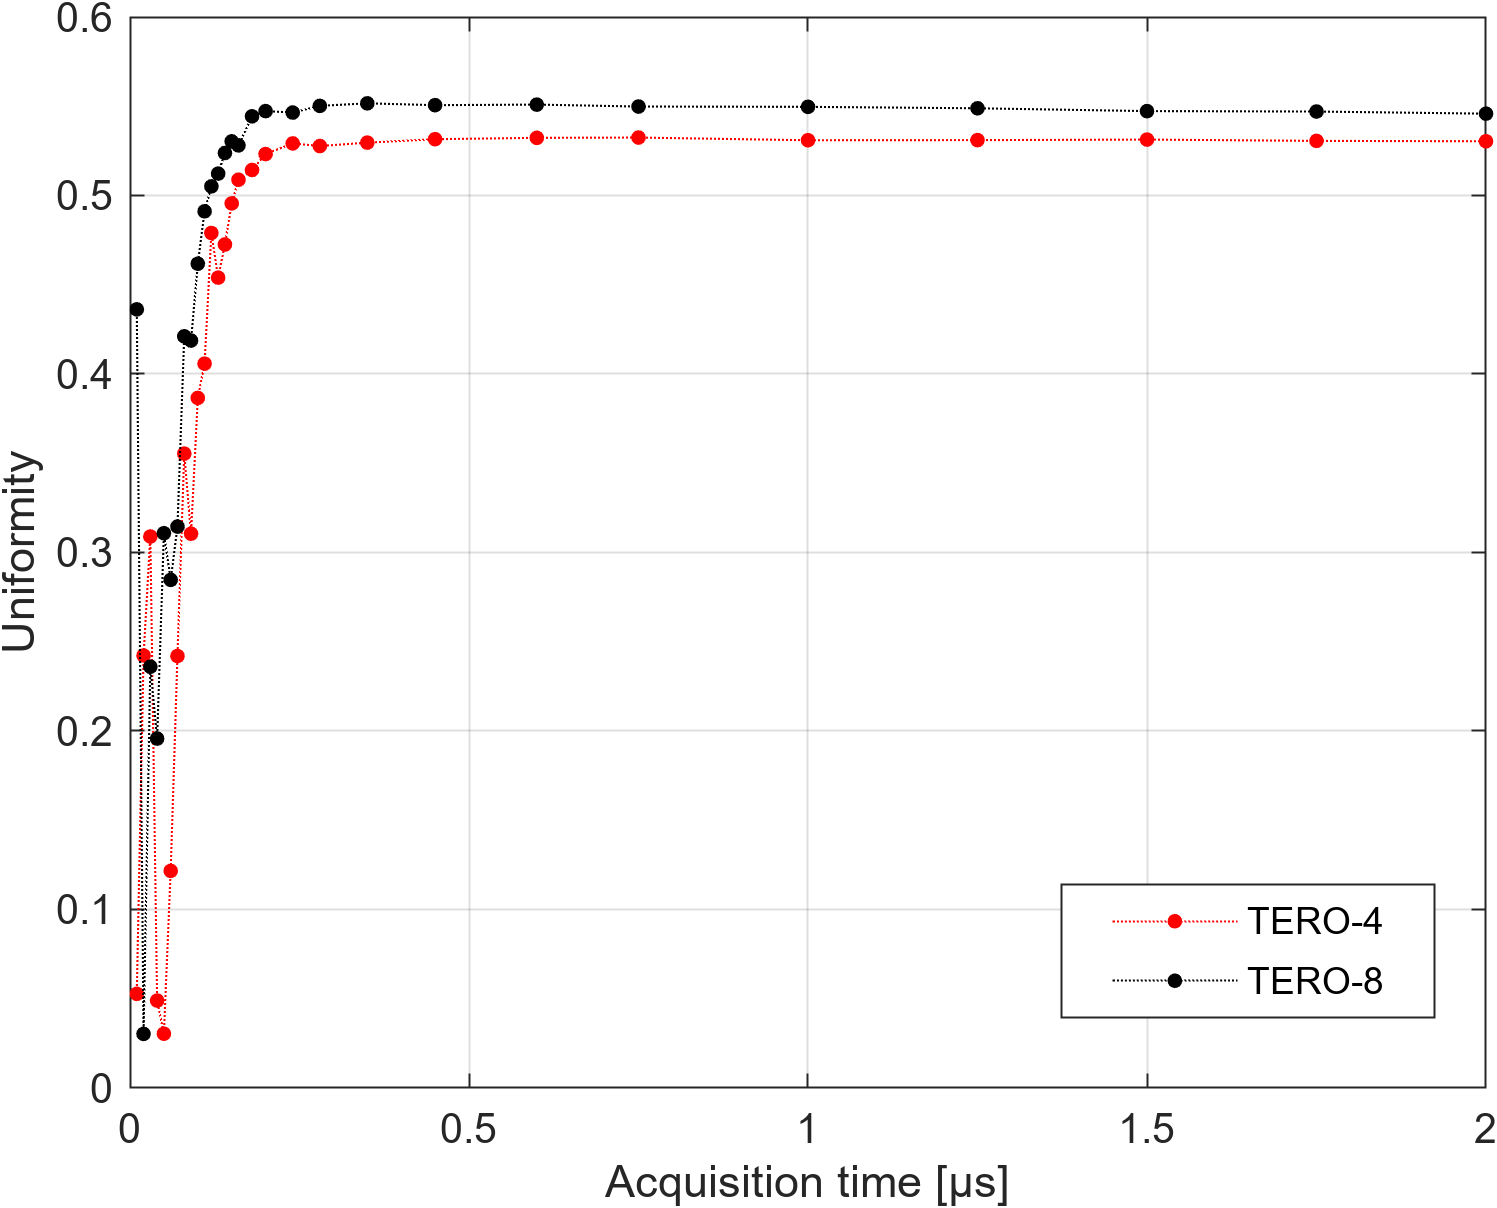
\includegraphics[width=\linewidth]
      {images/unlocked_tero_8_intra_uniformity.png}
      \subcaption{Uniformity}
   \end{minipage}\hfill
   \begin{minipage}[b]{0.50\linewidth}   
      \centering \includegraphics[width=\linewidth]{images/unlocked_tero_8_intra_reliability.png}
      \subcaption{Reliability}
   \end{minipage}
   \caption{\label{fig:locked_improvement_tero_8}TERO-8 performance improvement using locked pin}
\end{figure}

\newpage
\section{LSFR combinations distribution}
\label{appendix:lsfr}

The LSFR is used to generate the combinations of cells to compare instead of storing them in memory. It ensures that all the combinations are covered exactly once except the '0-0' combination never generated, providing a uniform usage of each cell. However, this does not ensure that the cell usage stays as uniform as possible during the generation process, and it can be seen in figure~\ref{fig:cell_occurence} that it is indeed not completely uniform when only a part of the combination is generated. 


\begin{figure}[H]
    \centering
    \includegraphics[width=0.7\linewidth]{images/cell_occurence_171.png}
    \caption{LSFR10 cells selection for only 171 bits}
    \label{fig:cell_occurence}
\end{figure}

This means that some cells are more used than others for comparison in this case. If those cells have an extreme final state (high or low number of oscillations in regard to the other), the comparisons with those cells will almost always generate the same bit. Since this cell is used more often, this could have a negative impact on the uniformity of the response.

\begin{table}[H]  
  \centering
    \begin{tabular}{|c|c|c|c|c|c|}
        \hline
        \textbf{TERO-8} & Response size & Uniformity & Reliability & Bit-aliasing & Uniqueness\\
        \hline
        Full & 1023 bits & 53.4\% & 97.6\% & 53.5\% & 49.4\%\\
        \hline
        Reduced & 171 bits & 53.4\% &97.7\% & 54.4\% & 49.9\%\\
        \hline
    \end{tabular}
   \caption{\label{tab:inter_perf_full_vs_reduce}TERO-8 performances for full and reduced response}
\end{table}

However, as we can see on the table~\ref{tab:inter_perf_full_vs_reduce}, this does not seem to have a significant impact on average on the TERO-8 implementation.

\newpage
\section{Python module}
\label{appendix:python_mod}

A Python module has been written to implement the UART interfaces in an easy-to-use method way. It used the \textbf{Pyserial} package for UART communication and \textbf{Numpy} to retrieve the data.

The PUF device is represented by the \textbf{PUF} class, which requires the port for the UART to be instantiated. We can also specify the baudrate and the initial value for the reference counter (to select the acquisition time).\\

Each interface with the PUF corresponds to a method:

\begin{itemize}
    \item \textbf{set\_ref\_limit(limit: int)}: update the limit of the reference counter, to change the acquisition time. The possible values are [1 -> 65536].
    \item \textbf{read\_raw()}: return the raw PUF response (1023 bits).
    \item \textbf{read\_ecc()}: return the PUF response after the BCH decoder (171 bits). The syndrome needs to be previously set using \textbf{set\_syndrome(syndrome: str)}.
    \item \textbf{read\_sha()}: return the sha256 key (256 bits).
\end{itemize}


For each reading operation, a second method has been created to easily record multiple samples for the same test. The return of those methods has their own class \textbf{SamplesReturnData} that stores the responses samples and computes the corresponding reference response and uniformity. This could easily be extended to also compute the reliability.

A second point that could be improved would be to compute the syndrome from the raw PUF response directly on this module instead of using Matlab. It could therefore automatically do the provision step at start then send the syndrome each time it is needed.



  





\end{document}